\documentclass[uplatex,b5paper]{jsreport}

\usepackage[dvipdfmx]{graphicx}
\usepackage[dvipdfmx]{hyperref}
\usepackage[]{pxjahyper}
\usepackage[]{textcomp}

\hypersetup{
  setpagesize = false,
    bookmarksnumbered = true,%
    bookmarksopen = true,%
    colorlinks = true,%
    linkcolor = black,
    citecolor = black,
    urlcolor = blue,
}


\title{2021 Geologie-Exkursionsbericht}
\author{}
\date{}

\begin{document}
  \maketitle
%  \begin{abstract}
%    test
%  \end{abstract}
  \tableofcontents
  \clearpage
  \chapter{はじめに}
    % Eine Er\"{o}rterung der Geologie und Stratigraphie der einzelnen Standorte in Bezug auf die am 21. Oktober 2021 durchgef\"{u}hrten geologischen Feldarbeiten.  \\
    本校では,実際の自然を観察,調査することで授業で学習している事柄に関する知見をより深める事を目的として,40年以上にわたり毎年地学野外実習を行っている。本稿では,令和3年10月21日に大阪府貝塚市蕎原において行われた同実習について,各地点の地形及び地層に関する考察を行う。
    
    各地点のまとめ方については,地点ごとに
    \begin{enumerate}
      \item 基本情報(岩石の種類,走向傾斜,特徴的な地形など)
      \item 観察冊子の各設問への回答\footnote{走向を測定するといった設問については基本情報に記すことで省いている場合がある。}
      \item 設問等を踏まえての考察\footnote{考察を記せていないものもある。}
    \end{enumerate}
    の3つを基本として1~2ページにまとめている。また,写真がある地点については写真を添付している。

    授業で扱わなかった用語等に関しては脚注に説明(多くは引用)を付している。なお,引用時に次の書籍については略記する\par
    ・ニューステージ地学図表(浜島書店,2013):図表

  \chapter{各地点}
  \clearpage

  \section{地点1}
    \subsection{基礎情報}
    岩石:泉南流紋岩(1億年前~9,000万年前)\par
    特徴:柱状節理\par
    \subsection{設問}
    \leftline{\large \textbf{◎この露頭を構成している岩石を調べる。}}
      \paragraph{ハンマーで叩いて,岩石の中の色と表面の色を比べる。表面の色と中の色が違うのはなぜか? どちらが本当の色か?}
      表面は茶色がかっているが,中は緑色と白色をしている。なお,割った際に赤色がみられることがあるが,これは酸化によるものと考えられる。
      \paragraph{どのような鉱物が含まれているか?またその鉱物の形状は?}
      白色であることから,長石や石英が含まれていると考えられる。
      \paragraph{これは堆積岩か,火成岩か,変成岩か?}
      斑状組織が見られ,石英や長石を含むことから火成岩,特に火山岩であることがうかがえる。
      \paragraph{さらに詳しくみて,これは何岩か?}
      火山岩のうち,石英や長石(無色鉱物)を多く含むのは流紋岩である。よって\textbf{この岩石は泉南流紋岩であると考えられる。}
  \begin{figure}[h]
    \begin{center}
      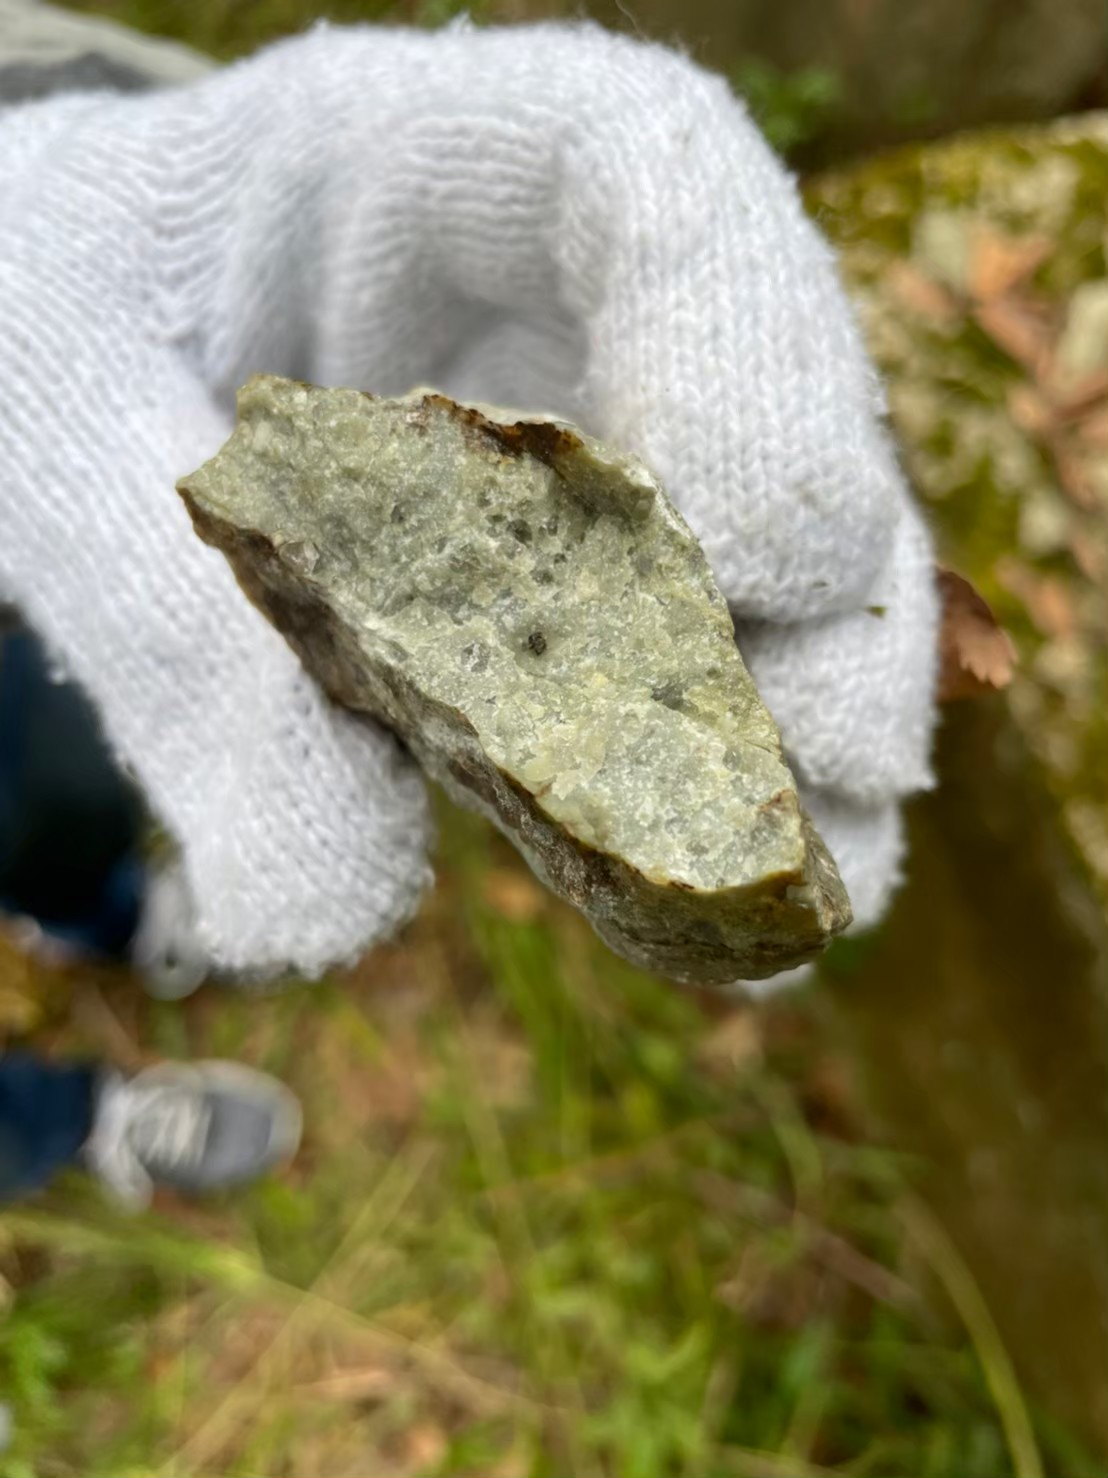
\includegraphics[scale=0.12]{files/地学実習/泉南流紋岩.jpg}
      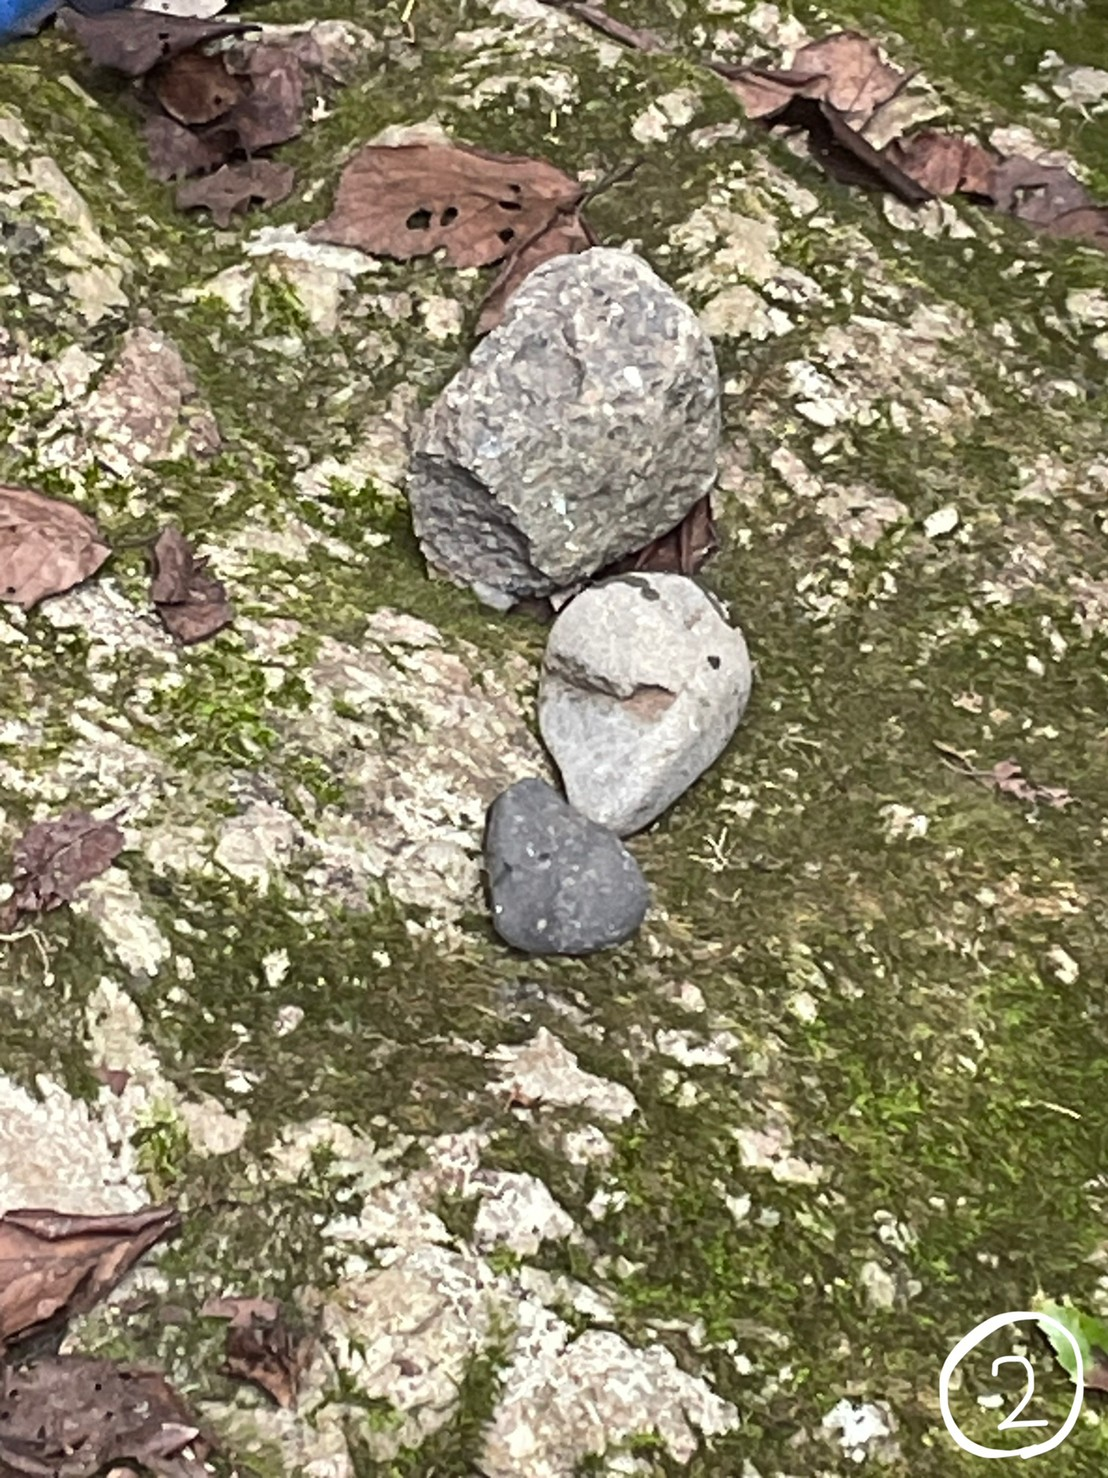
\includegraphics[scale=0.12]{files/地学実習/泉南流紋岩_2.jpg}
      \caption{泉南流紋岩}
    \end{center}
  \end{figure}

    \leftline{\large \textbf{◎崖に見られる割れ目は何か}}
    柱状節理(後述)
    \subsection{考察}
    観察した崖は中央のみが削れており,それに対して両側は削れずに木も生えていた。これは,中央に断層が走っておりそこで地震が発生したためと考えられる。また,崖の岩石は亀裂が入っているが,これは\textbf{節理}\footnote{「柱状節理 溶岩が冷却される際に収縮して,柱状に割れ目(節理)が形成されたもの。玄武岩などに見られる。節理は冷却面と垂直に発達する。」―図表p.105}であると考えられ,亀裂の入り方から柱状節理の可能性が高い。
  \clearpage

  \section{地点2}
    \subsection{基本情報}
    岩石:泉南流紋岩(1億年前~9,000万年前)\par
    走向:N30\textdegree E\par
    傾斜:90\textdegree N\par
    \subsection{設問}
    \leftline{\large \textbf{◎この露頭を構成する岩石は?}}
    色味などから,泉南流紋岩と考えられる。\par
    \leftline{\large \textbf{◎この滝の成因について考える。}}
      \paragraph{この付近に,特徴的な地形としてどのようなものが観察できるか。}
      水深が深い。大きなくぼみがある。
      \paragraph{上記地形は,どのようにしてできたと考えられるか?}
      断層の影響によるもの。
      \paragraph{対岸のくぼみは何か?}
      断層
      \begin{figure}[h]
        \begin{center}
          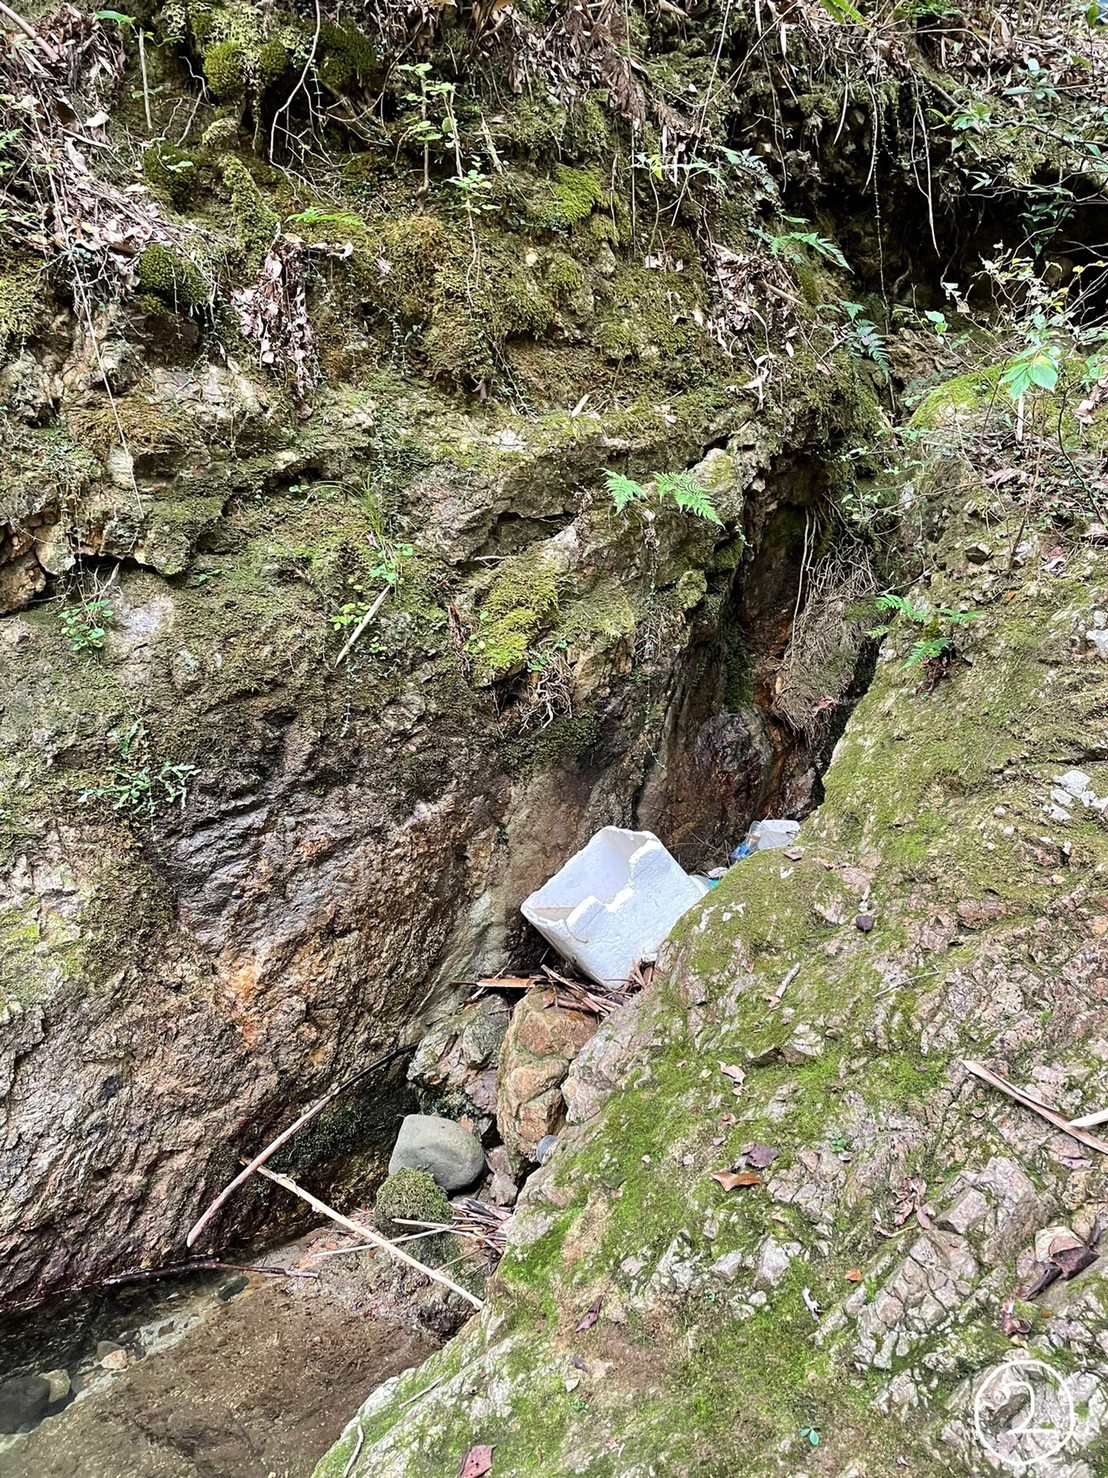
\includegraphics[scale=0.1]{files/地学実習/地点2_窪み.jpg}
          \caption{くぼみ}
        \end{center}
      \end{figure}
      \paragraph{くぼみに現れた面(断層面)の走向傾斜を測り,地図上に走向線を引く。その線上にはどのような地形がみられるか?}
      線の先には地点1がある。
      \paragraph{くぼみの幅も測っておく。}
    \subsection{考察}
    走向からみるに,地点1と地点2は同一の断層上にあると考えられる。
  \begin{figure}[h]
    \begin{center}
      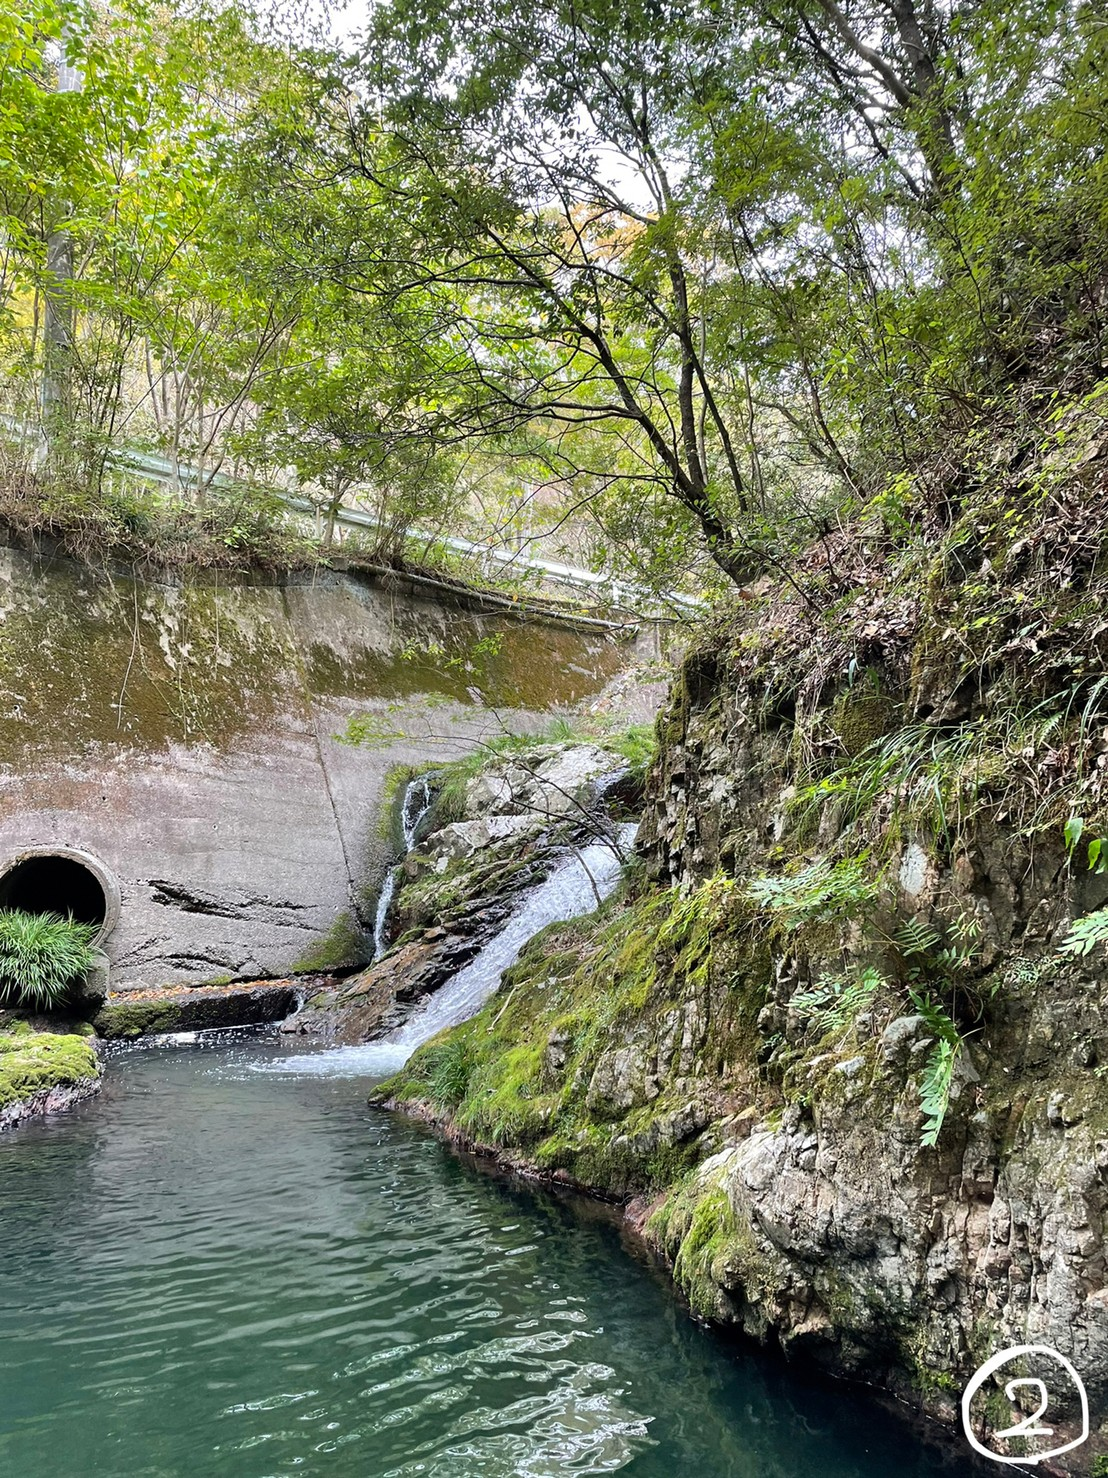
\includegraphics[scale=0.3]{files/地学実習/地点2.jpg}
      \caption{地点2}
    \end{center}
  \end{figure}
  \clearpage

  \section{地点3}
    \subsection{基本情報}
    岩石:断層粘土,泉南流紋岩\par
    走向:N40\textdegree E\par
    傾斜:70\textdegree N\par
    特徴:断層破砕帯
    \subsection{設問}
    \leftline{\large \textbf{◎露頭の中ほどの他と少し違う様子の違うところに注目。}}
      \paragraph{手で触ってみたり,ハンマーでたたいて手ごたえを調べる。これは何か。}
      柔らかく,触るとボロボロと崩れる。また,この地点は侵食,崩壊の具合から見て断層破砕帯\footnote{「断層面に沿ってできている岩石破砕部。(中略)粘土などから成る。破砕帯は一般に軟弱で,侵食,崩壊が早く進む。」「断層面に沿って周囲の岩石が破砕されている場合,その部分を断層破砕帯または単に破砕帯と呼ぶ。破砕帯が角ばった岩石の破片から構成されている場合,それを断層角礫と呼び,粘土状物質から構成されている場合は断層粘土と呼ぶ。」―コトバンク『断層破砕帯』}と考えられ,それらのことからこの岩石は断層粘土である。
      \paragraph{綺麗な面が出ているところで走向傾斜を測定し,地図上に走向線を引く。何か気付くことはないか?}
      地点3の断層と地点1,2の断層は全く別の断層である事が分かる。
    \subsection{考察}
    地点1,2と同じ泉南流紋岩でできた地層だがそれらとは異なる断層である。地形図から想定するに,この断層はこの地点を端として南西に続いていると考えられる。
  \begin{figure}[h]
    \begin{center}
      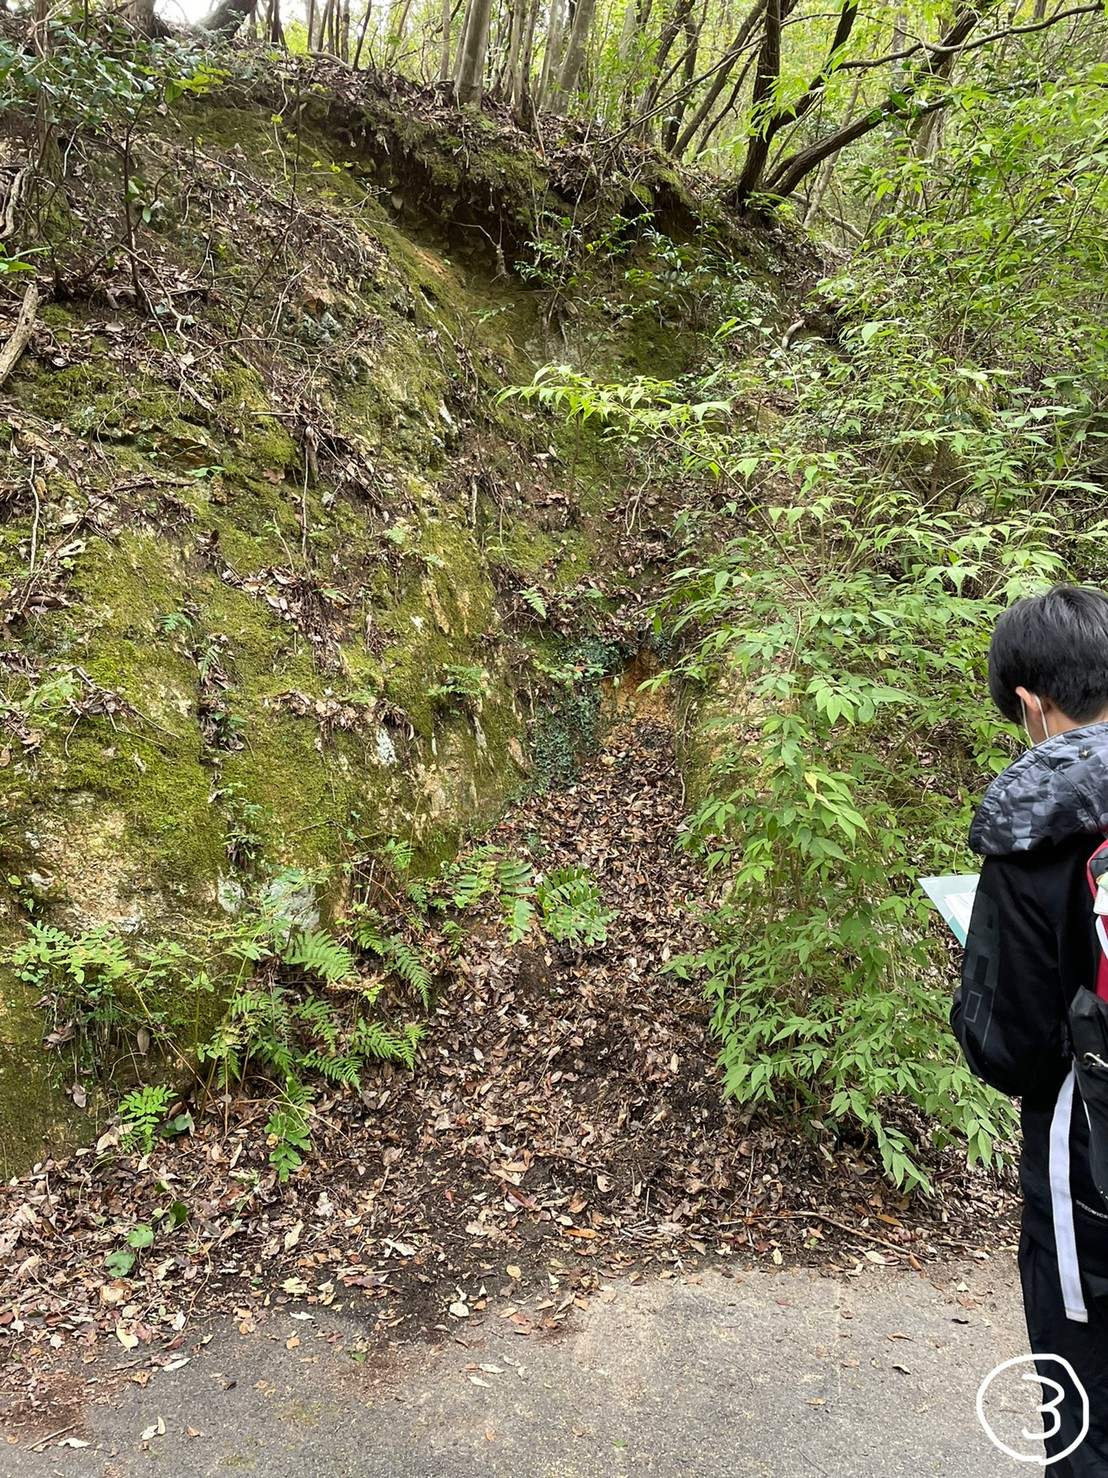
\includegraphics[scale=0.07]{files/地学実習/地点3.jpg}
      \caption{地点3}
    \end{center}
  \end{figure}
  \clearpage

  \section{地点4}
    \subsection{基本情報}
    岩石:泉南流紋岩(,断層粘土)\par
    走向:N55\textdegree E\par
    傾斜:65\textdegree N\par
    \subsection{設問}
    \leftline{\large \textbf{◎谷の奥のくぼみに注目。}}
      \paragraph{このくぼみは何か。予想を立てたらその証拠を探しに奥へ入る。何があるか。}
      湿っていることから破砕帯ではないかと考えた。
    \subsection{考察}
    湿っていることと崩れ気味なことから破砕帯である可能性を考えたが,断層粘土のような柔らかい岩石はほとんど見かけられないため確実とは言い難い。
    \begin{figure}[h]
      \begin{center}
        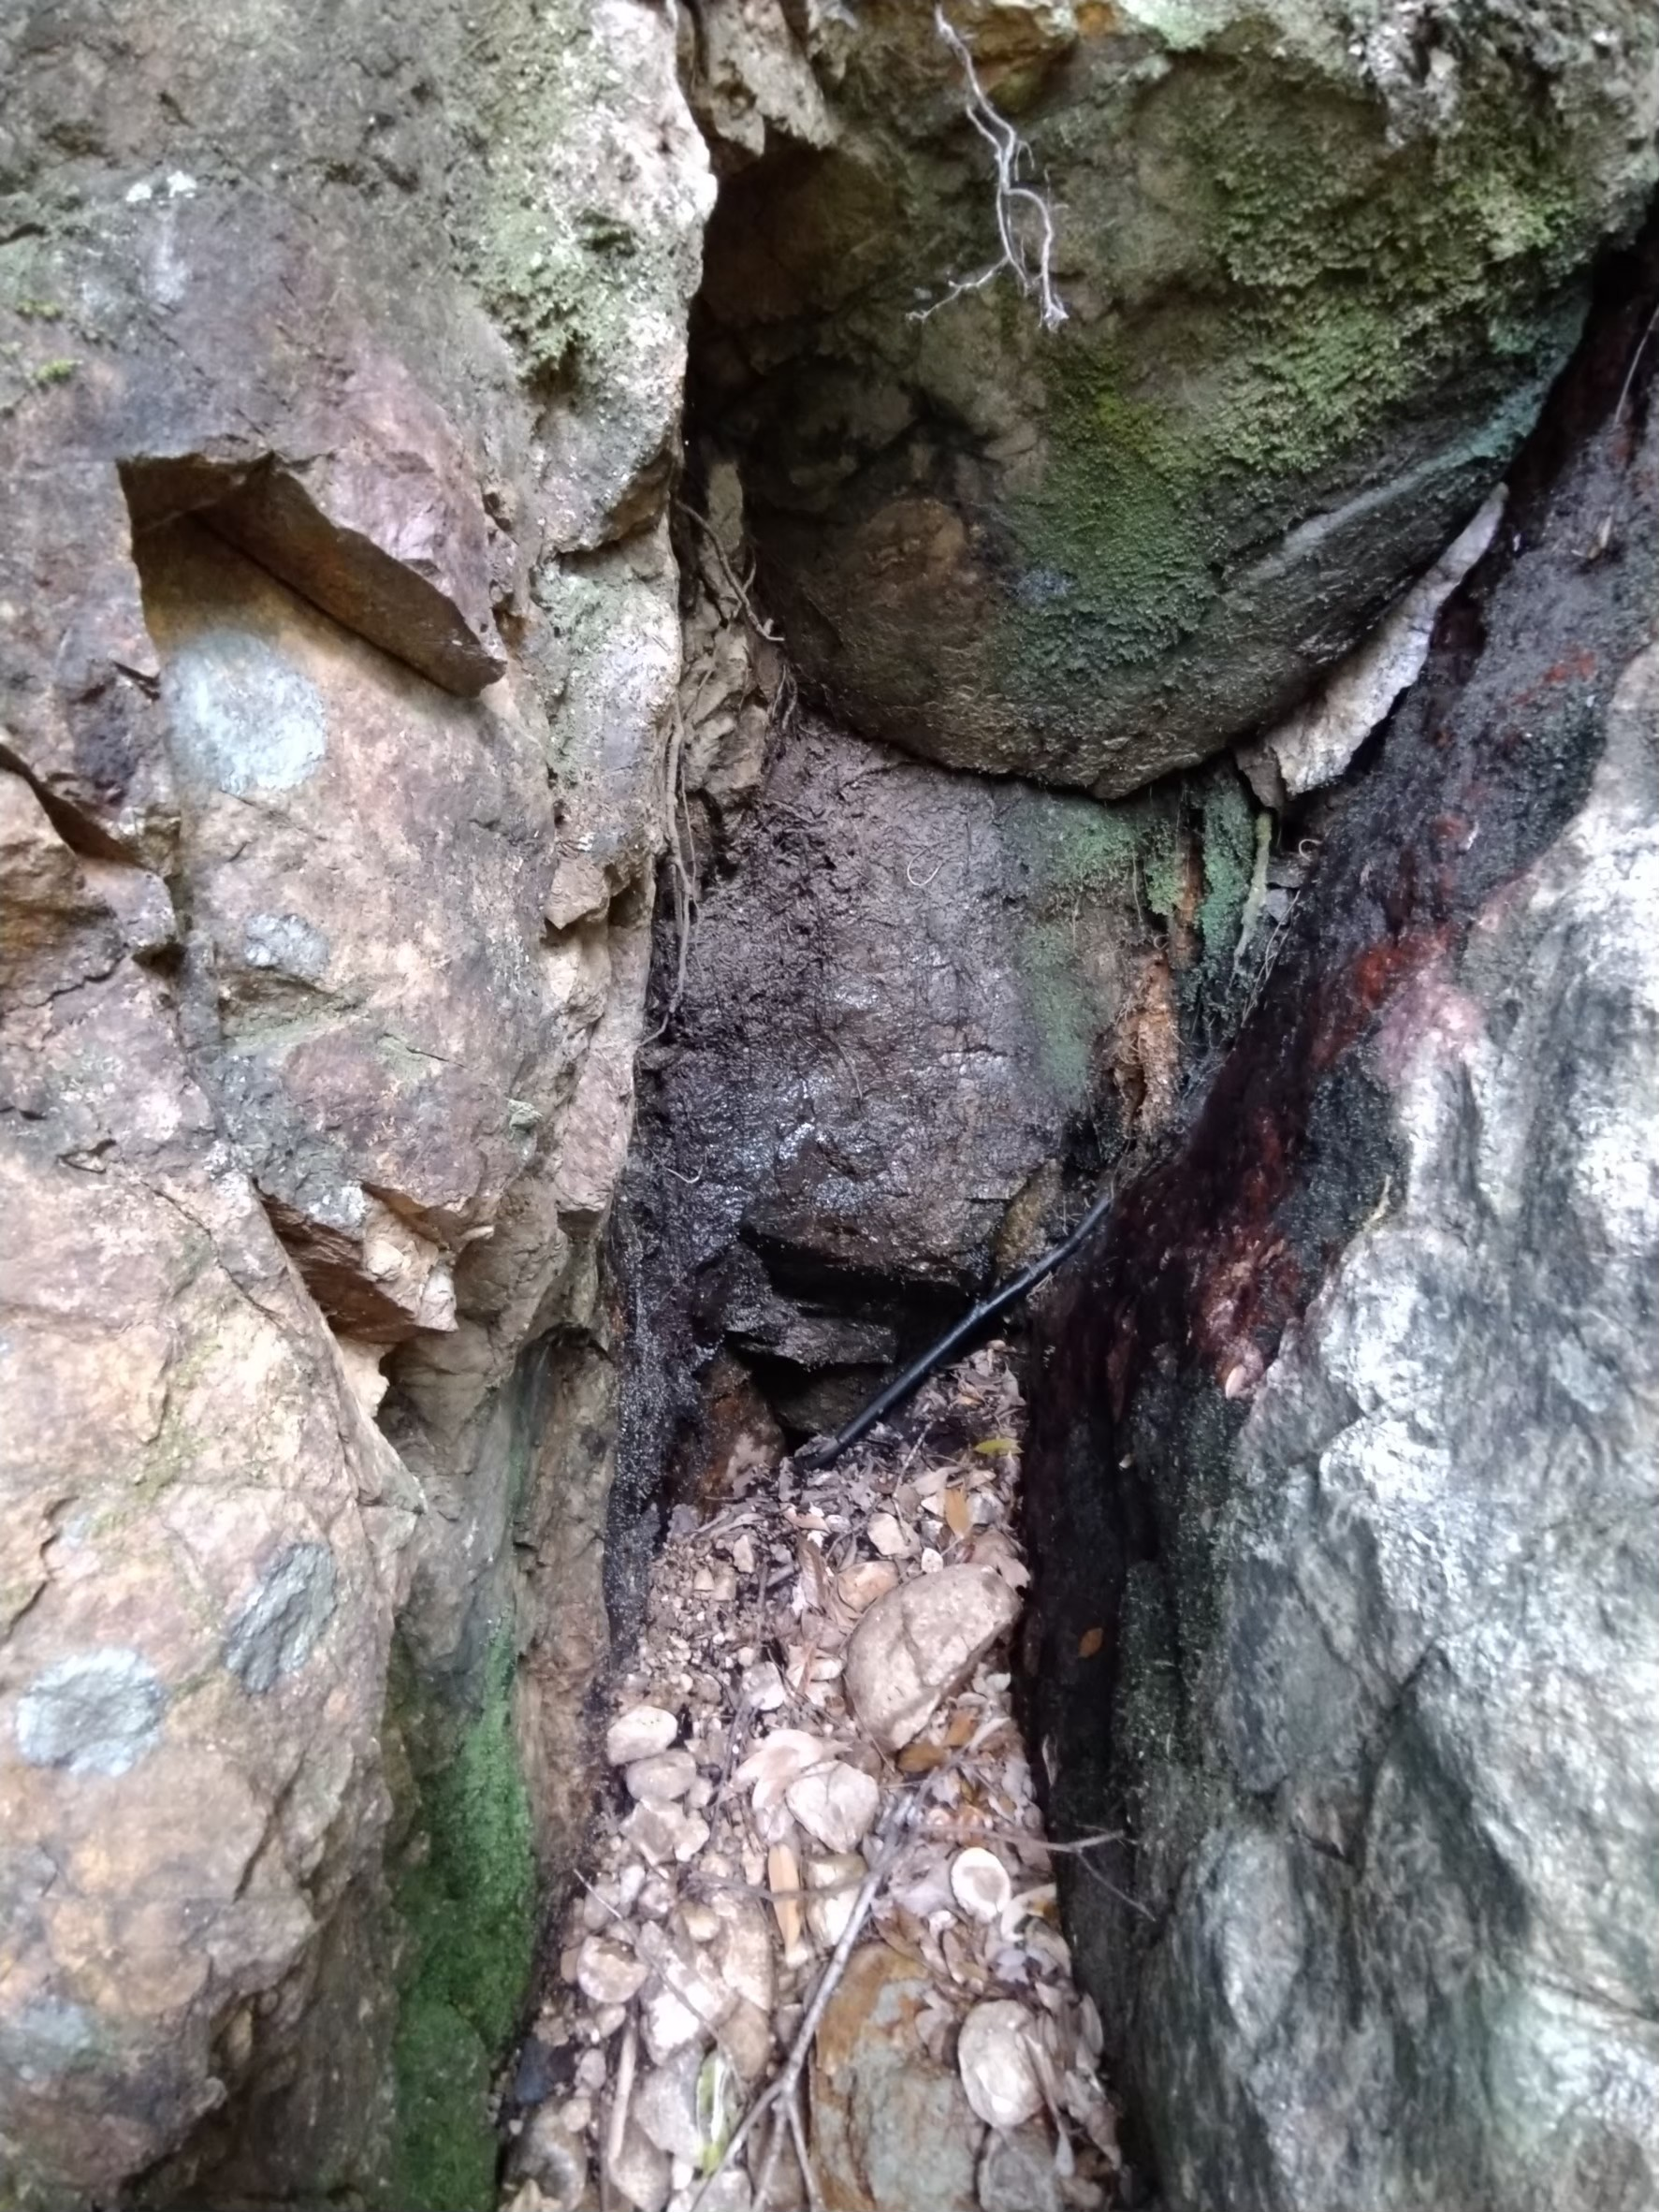
\includegraphics[scale=0.1]{files/地学実習/地点4.jpg}
        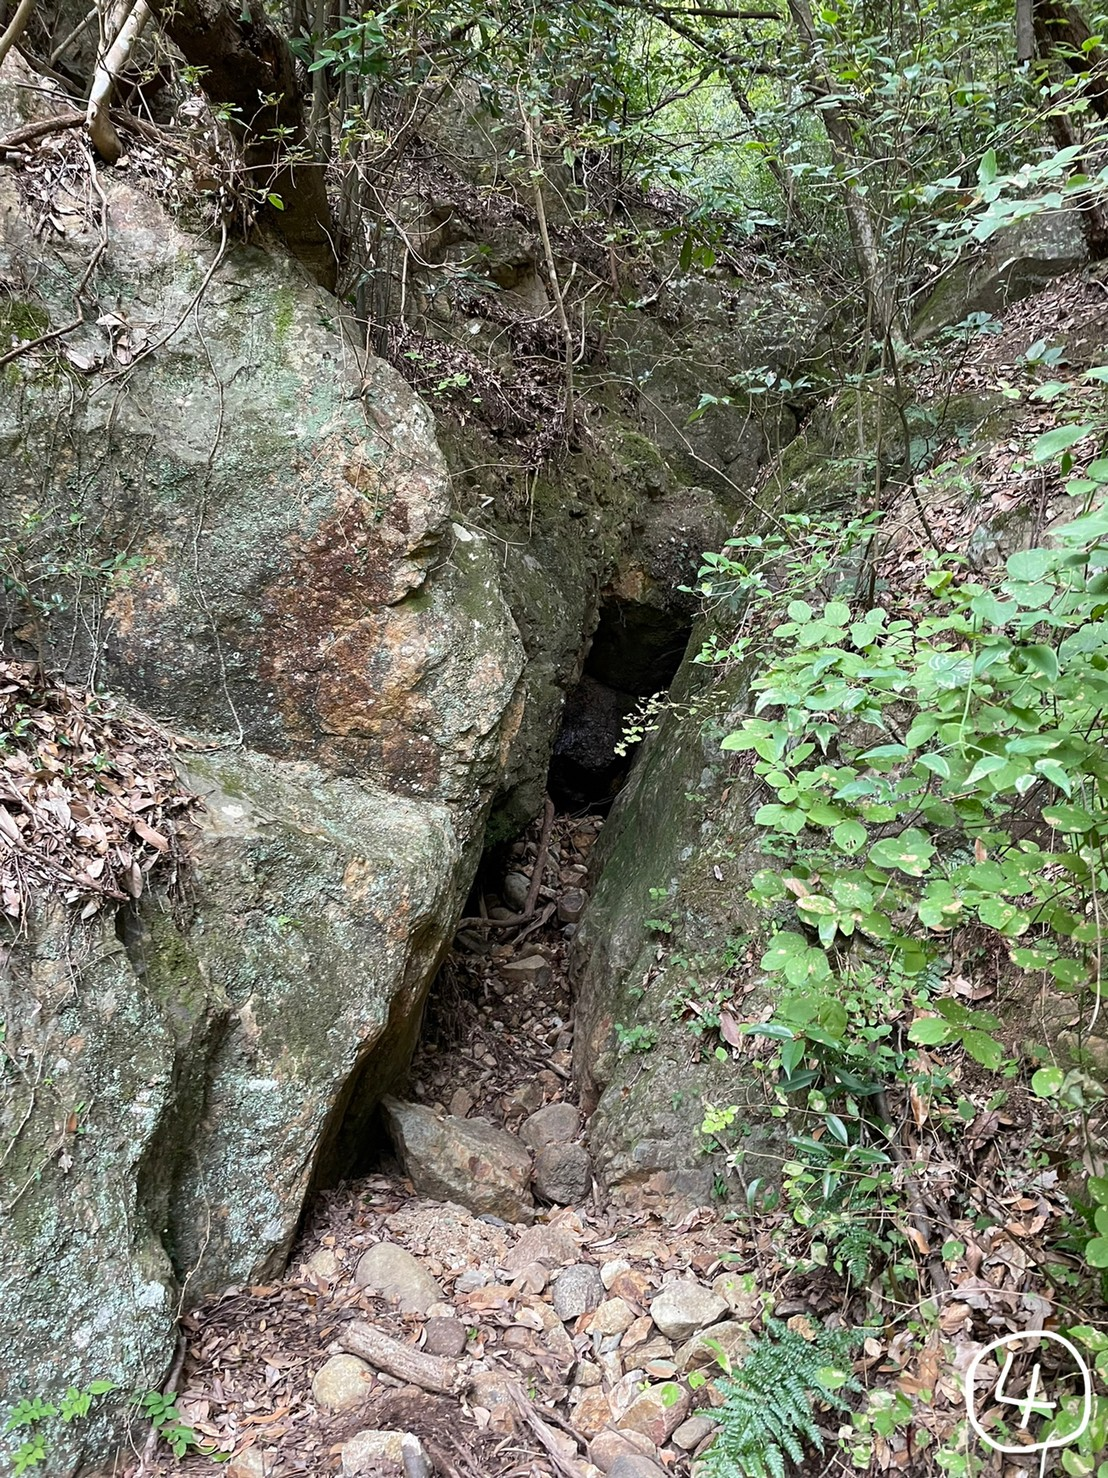
\includegraphics[scale=0.15]{files/地学実習/地点4_2.jpg}
        \caption{地点4}
      \end{center}
    \end{figure}
  \clearpage

  \section{地点5}
    \subsection{基本情報}
    岩石:礫岩,泉南流紋岩\par
    走向:N55\textdegree E\par
    傾斜:65\textdegree N\par
    特徴:和泉層群,基底礫岩,秋山不整合
    \subsection{設問}
    \leftline{\large \textbf{◎この露頭の構造について調べる。}}
      \paragraph{露頭を構成する岩石に注目。今までとの違いはないか?}
      今までは泉南流紋岩ばかりだったが,ここでは上側に礫岩がみられる。
      \paragraph{今までと同じ岩石(泉南流紋岩)がでているところはないか?}
      地層の下側には泉南流紋岩がみられる。
      \paragraph{その境目はないか?またその境目はどのように続いているか?}
      斜めに走った境目がある。境目は道路の向かいの地層にも続いており,西に向かって傾いている。
      \paragraph{境目はなんと呼ぶべきか?}
      見たところ,境目は不整合面である。秋山不整合\footnote{和泉層群と泉南流紋岩層との不整合面のことを一般に秋山不整合と呼ぶ。}だろう。
      \leftline{\large \textbf{◎礫の大きさ(最大径)や形,礫種を調べる。}}
      礫の大きさは140mm~150mmと大きめで,形は丸い。礫種は大礫\footnote{砕屑岩のうち大きさが2mm以上のものを礫と呼び,そのうち4mmまでのものを細礫,64mmまでのものを中礫,256mmまでのものを大礫,それ以上の大きさのものを巨礫と呼ぶ。―図表p.124表より}
      \begin{figure}[h]
        \begin{center}
          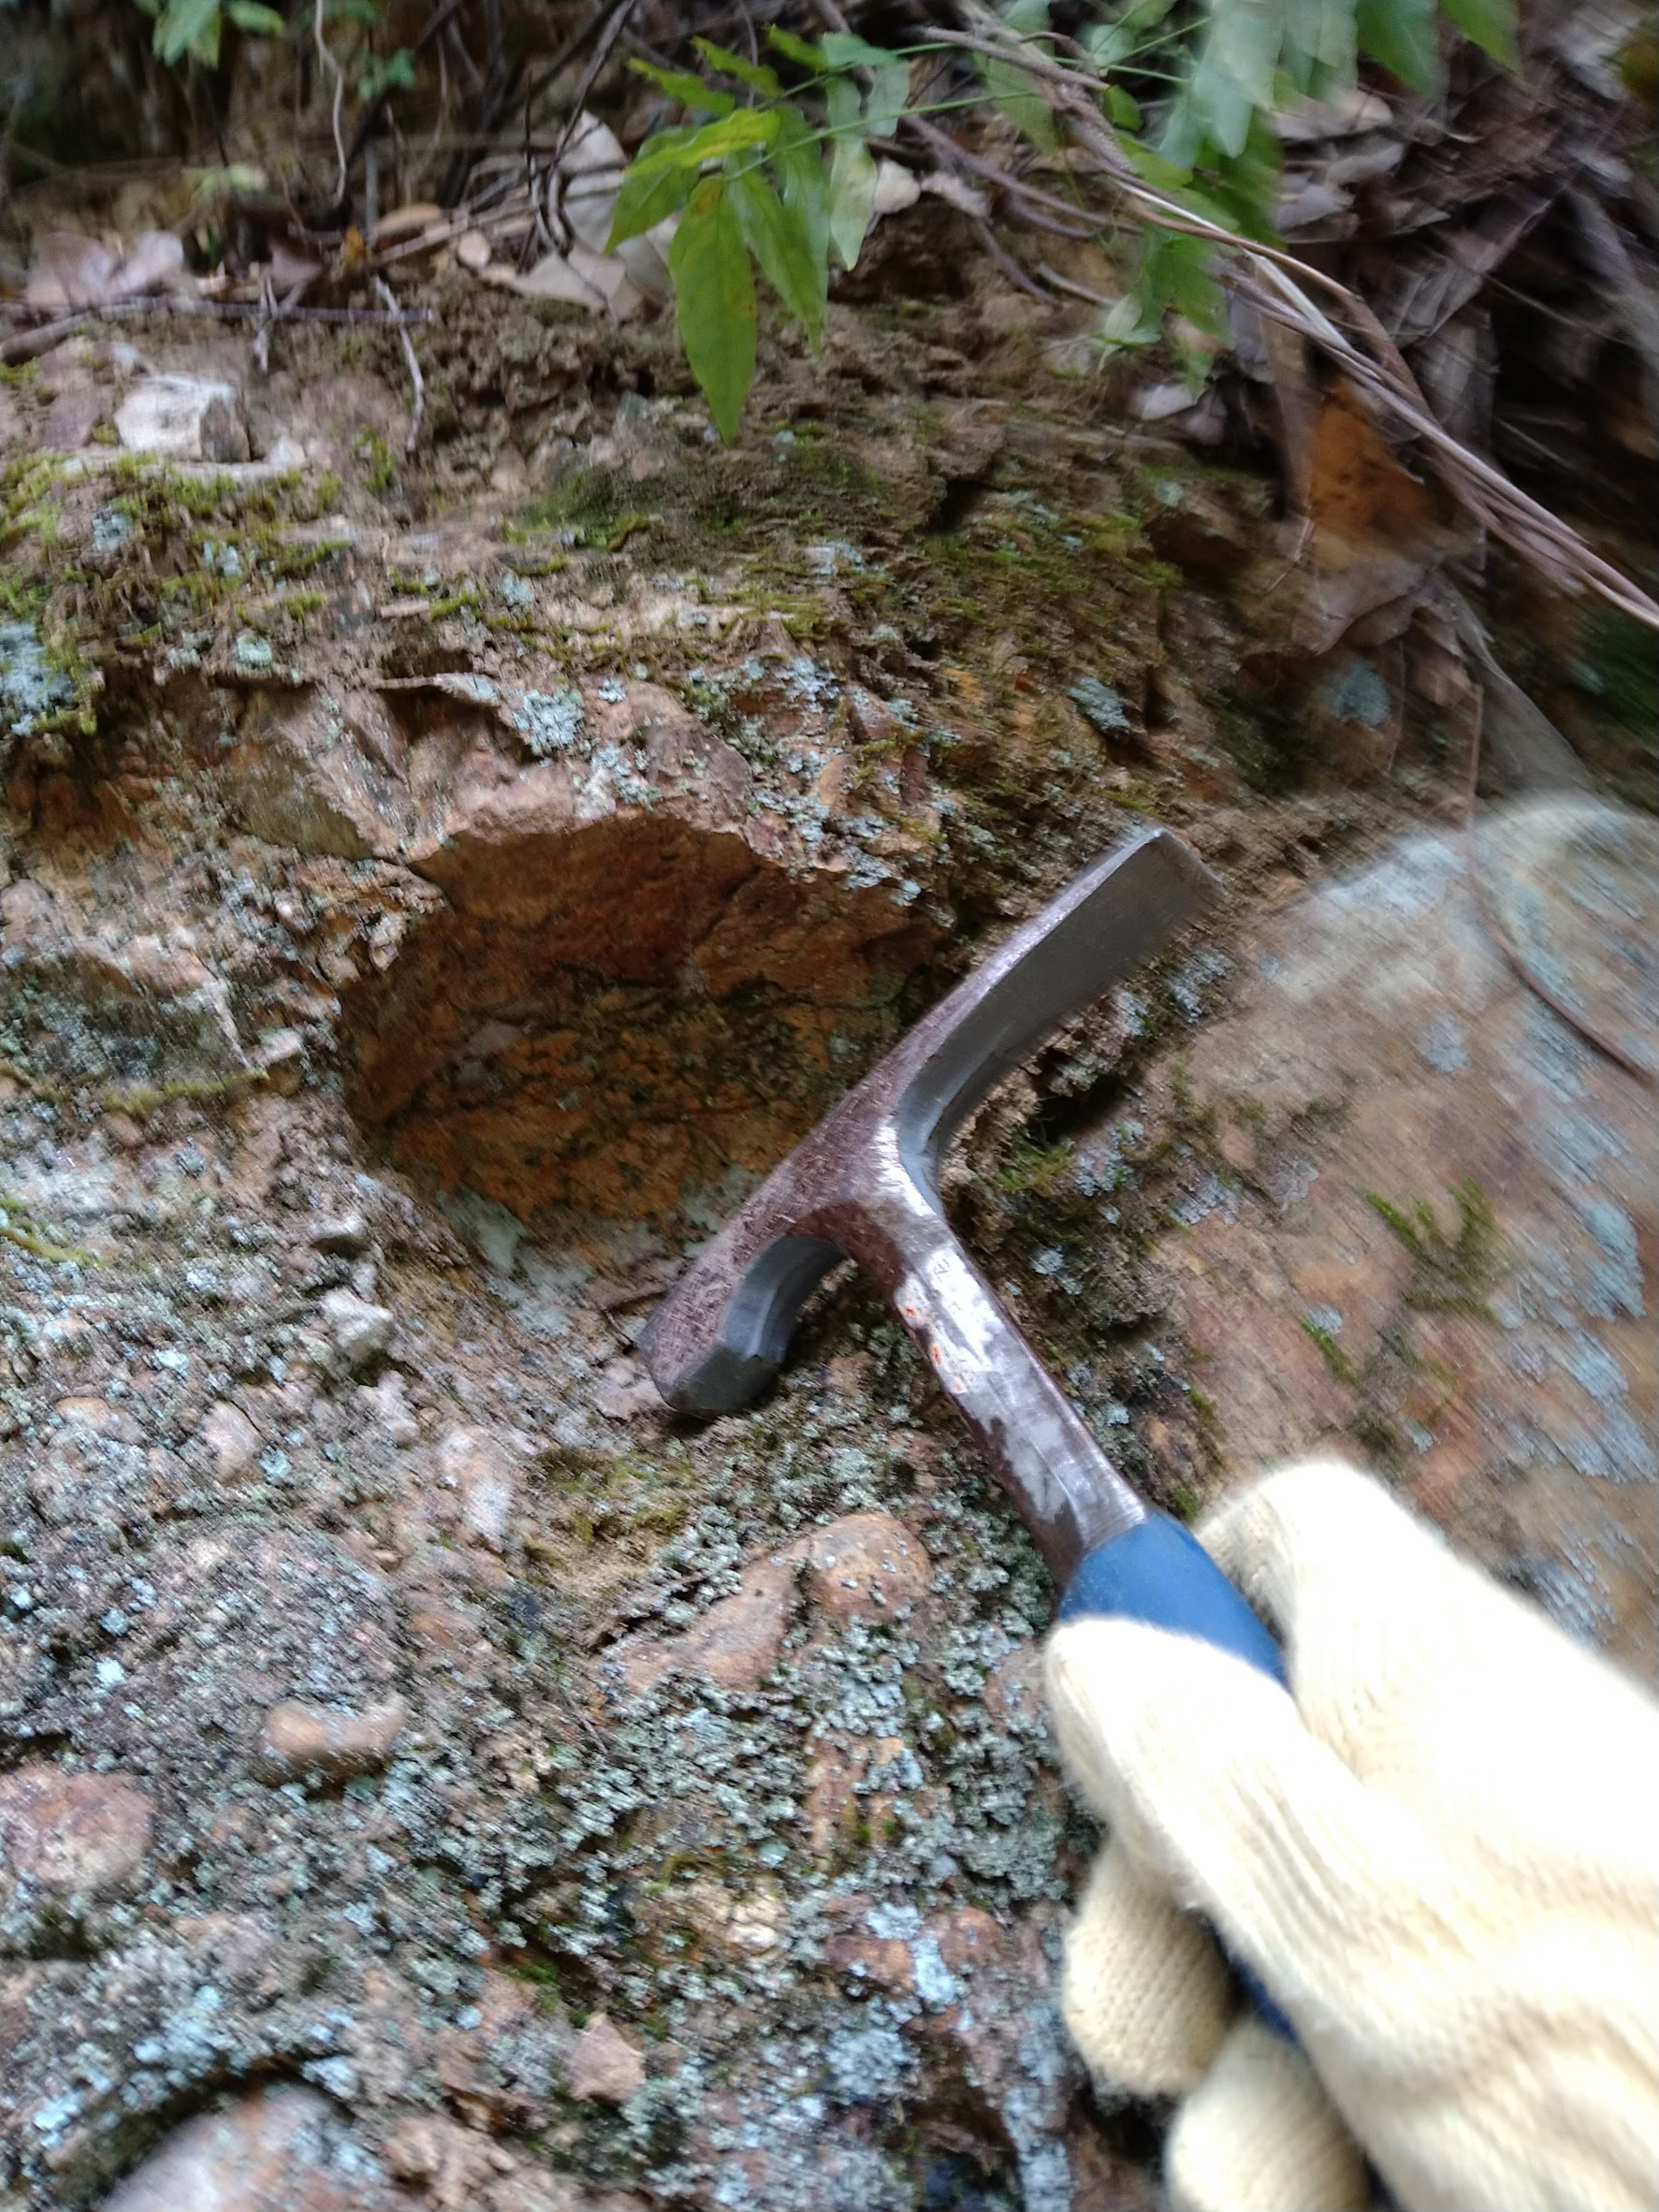
\includegraphics[scale=0.04]{files/地学実習/地点5_礫.jpg}
          \caption{礫(の穴)}
        \end{center}
      \end{figure}
    \subsection{考察}
    下側の泉南流紋岩と上側に積もっている礫岩の境目が不整合面であることから,上側の礫岩は基底礫岩\footnote{「不整合面のすぐ上には,粗粒な礫などが堆積することが多く,これを基底礫岩という。新旧2層の形成年代の間には長い時間間隔がある。」―図表p.128}であり,そうであるとすると2層の間には大きな年代差があり,また泉南流紋岩層は一度海に沈んでいたということになる。しかしその一方で,蕎原が和泉層群\footnote{「和泉層群は,中央構造線の北側にそって細長く分布している中生代白亜紀後期の地層です。(中略)この地層は主に海底で堆積した礫岩,砂岩,泥岩からなり,ところどころに酸性凝灰岩をはさんでいます。」―徳島の自然と歴史ガイドNo.3 和泉層群}の一部であることを踏まえると上側の礫岩は和泉層群の一部であると考えられること,泉南流紋岩,和泉層群ともに白亜紀の地層であることを留意されたい。
  \begin{figure}[h]
    \begin{center}
      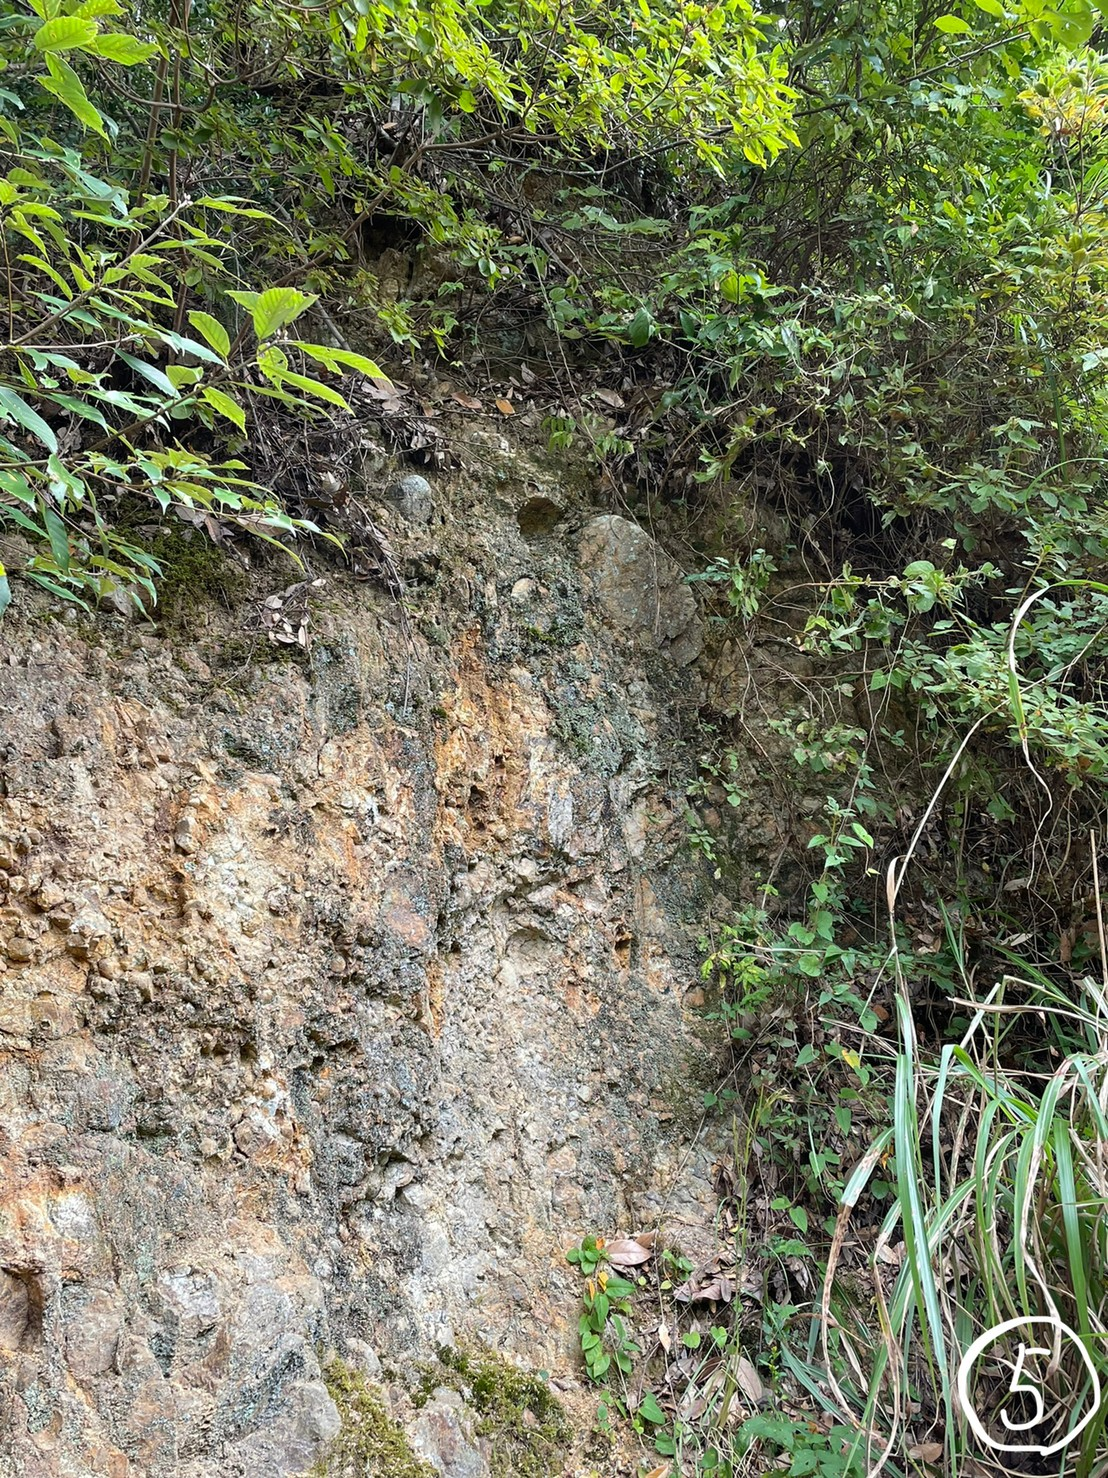
\includegraphics[scale=0.2]{files/地学実習/地点5.jpg}
      \caption{地点5}
    \end{center}
  \end{figure}
  \clearpage

  \section{地点6}
    \subsection{基本情報}
    岩石:礫岩 \par
    特徴:逆級化層理
    \subsection{設問}
    \leftline{\large \textbf{◎露頭に現れた礫に注目。}}
      \paragraph{地点5との違いはどこか?}
      泉南流紋岩が無くなり,礫岩のみとなった。
      \paragraph{礫の大きさ,形,礫種を調べる。}
      下の方が小さく,上に行くほど大きくなる。形は丸く,大きさは50mm程のもの(大礫)などがあった。
      \paragraph{なぜこのような違いが生じたのか,考えてみる。}
      大礫から成る地層であることも勘案すると,地点6は扇状地のような堆積地形であった可能性が考えられる。\footnote{「扇状地の堆積物は,淘汰(とうた)の悪い大礫や中礫が主体で,砂,シルト,粘土などは従属的である。礫は扇頂部に粗粒で,扇端部にいくにつれて細粒となる。堆積物の厚さは扇頂部よりむしろ扇央部に厚いことが多い。」―コトバンク『扇状地』}
    \subsection{考察}
    この地層は逆級化層理\footnote{「下部には粗粒な粒子,上部ほど細粒な粒子から成る地層を\textbf{級化層理(級化成層・級化構造)}という。時間とともに運搬する水流が弱くなったときなどに生じる。また,乱泥流などによって運ばれて堆積した場合にも生じる。地層の上下判定に役立つ。」―図表p.127 逆級化層理は級化層理の逆版である。}で,このようになった原因としてはブラジルナッツ効果\footnote{異なる大きさからなる粉粒体を振ると,最も大きな粒子が表面に浮き上がってくる現象。}が考えられる。
  \begin{figure}[h]
    \begin{center}
      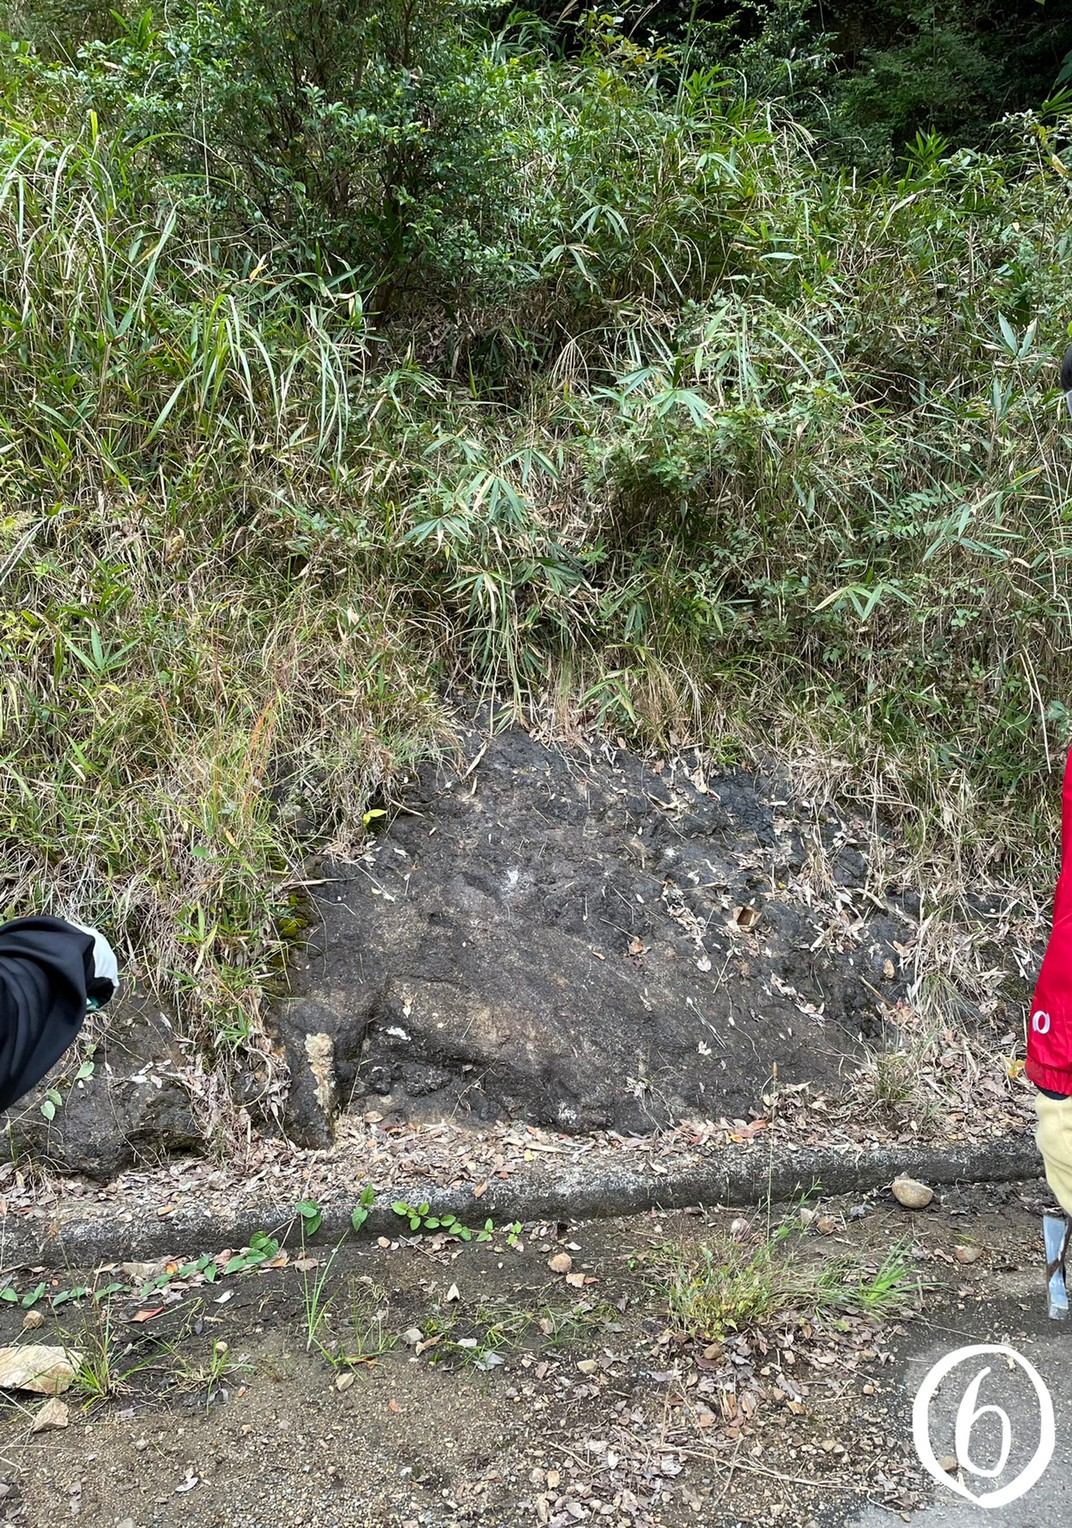
\includegraphics[scale=0.06]{files/地学実習/地点6.jpg}
      \caption{地点6}
    \end{center}
  \end{figure}
  \clearpage

  \section{地点7}
    \subsection{基本情報}
    岩石:砂岩,礫岩
    特徴:隆起,沈降
    \subsection{設問}
    \leftline{\large \textbf{◎小屋の裏の斜面に注目。}}
      \paragraph{この露頭に見られる特徴的な構造は?}
      礫岩と砂岩が交互に重ね合わさっている構造。
      \paragraph{ひとつの単層に注目。どのように続いているか?}
      北の方が高く,南の方が低い。
      \paragraph{この地層にどのような力が働いたと考えられるか?}
      この地層が海底にあった際に海底が隆起と沈降を繰り返したため,このような地層になった。
    \subsection{考察}
    写真で見える限りでも礫<砂<礫<砂<礫となっているので,少なくとも4回は隆起・沈降が起こっていることが分かる(実際の回数はもっと多いと思われる。)。
  \begin{figure}[h]
    \begin{center}
      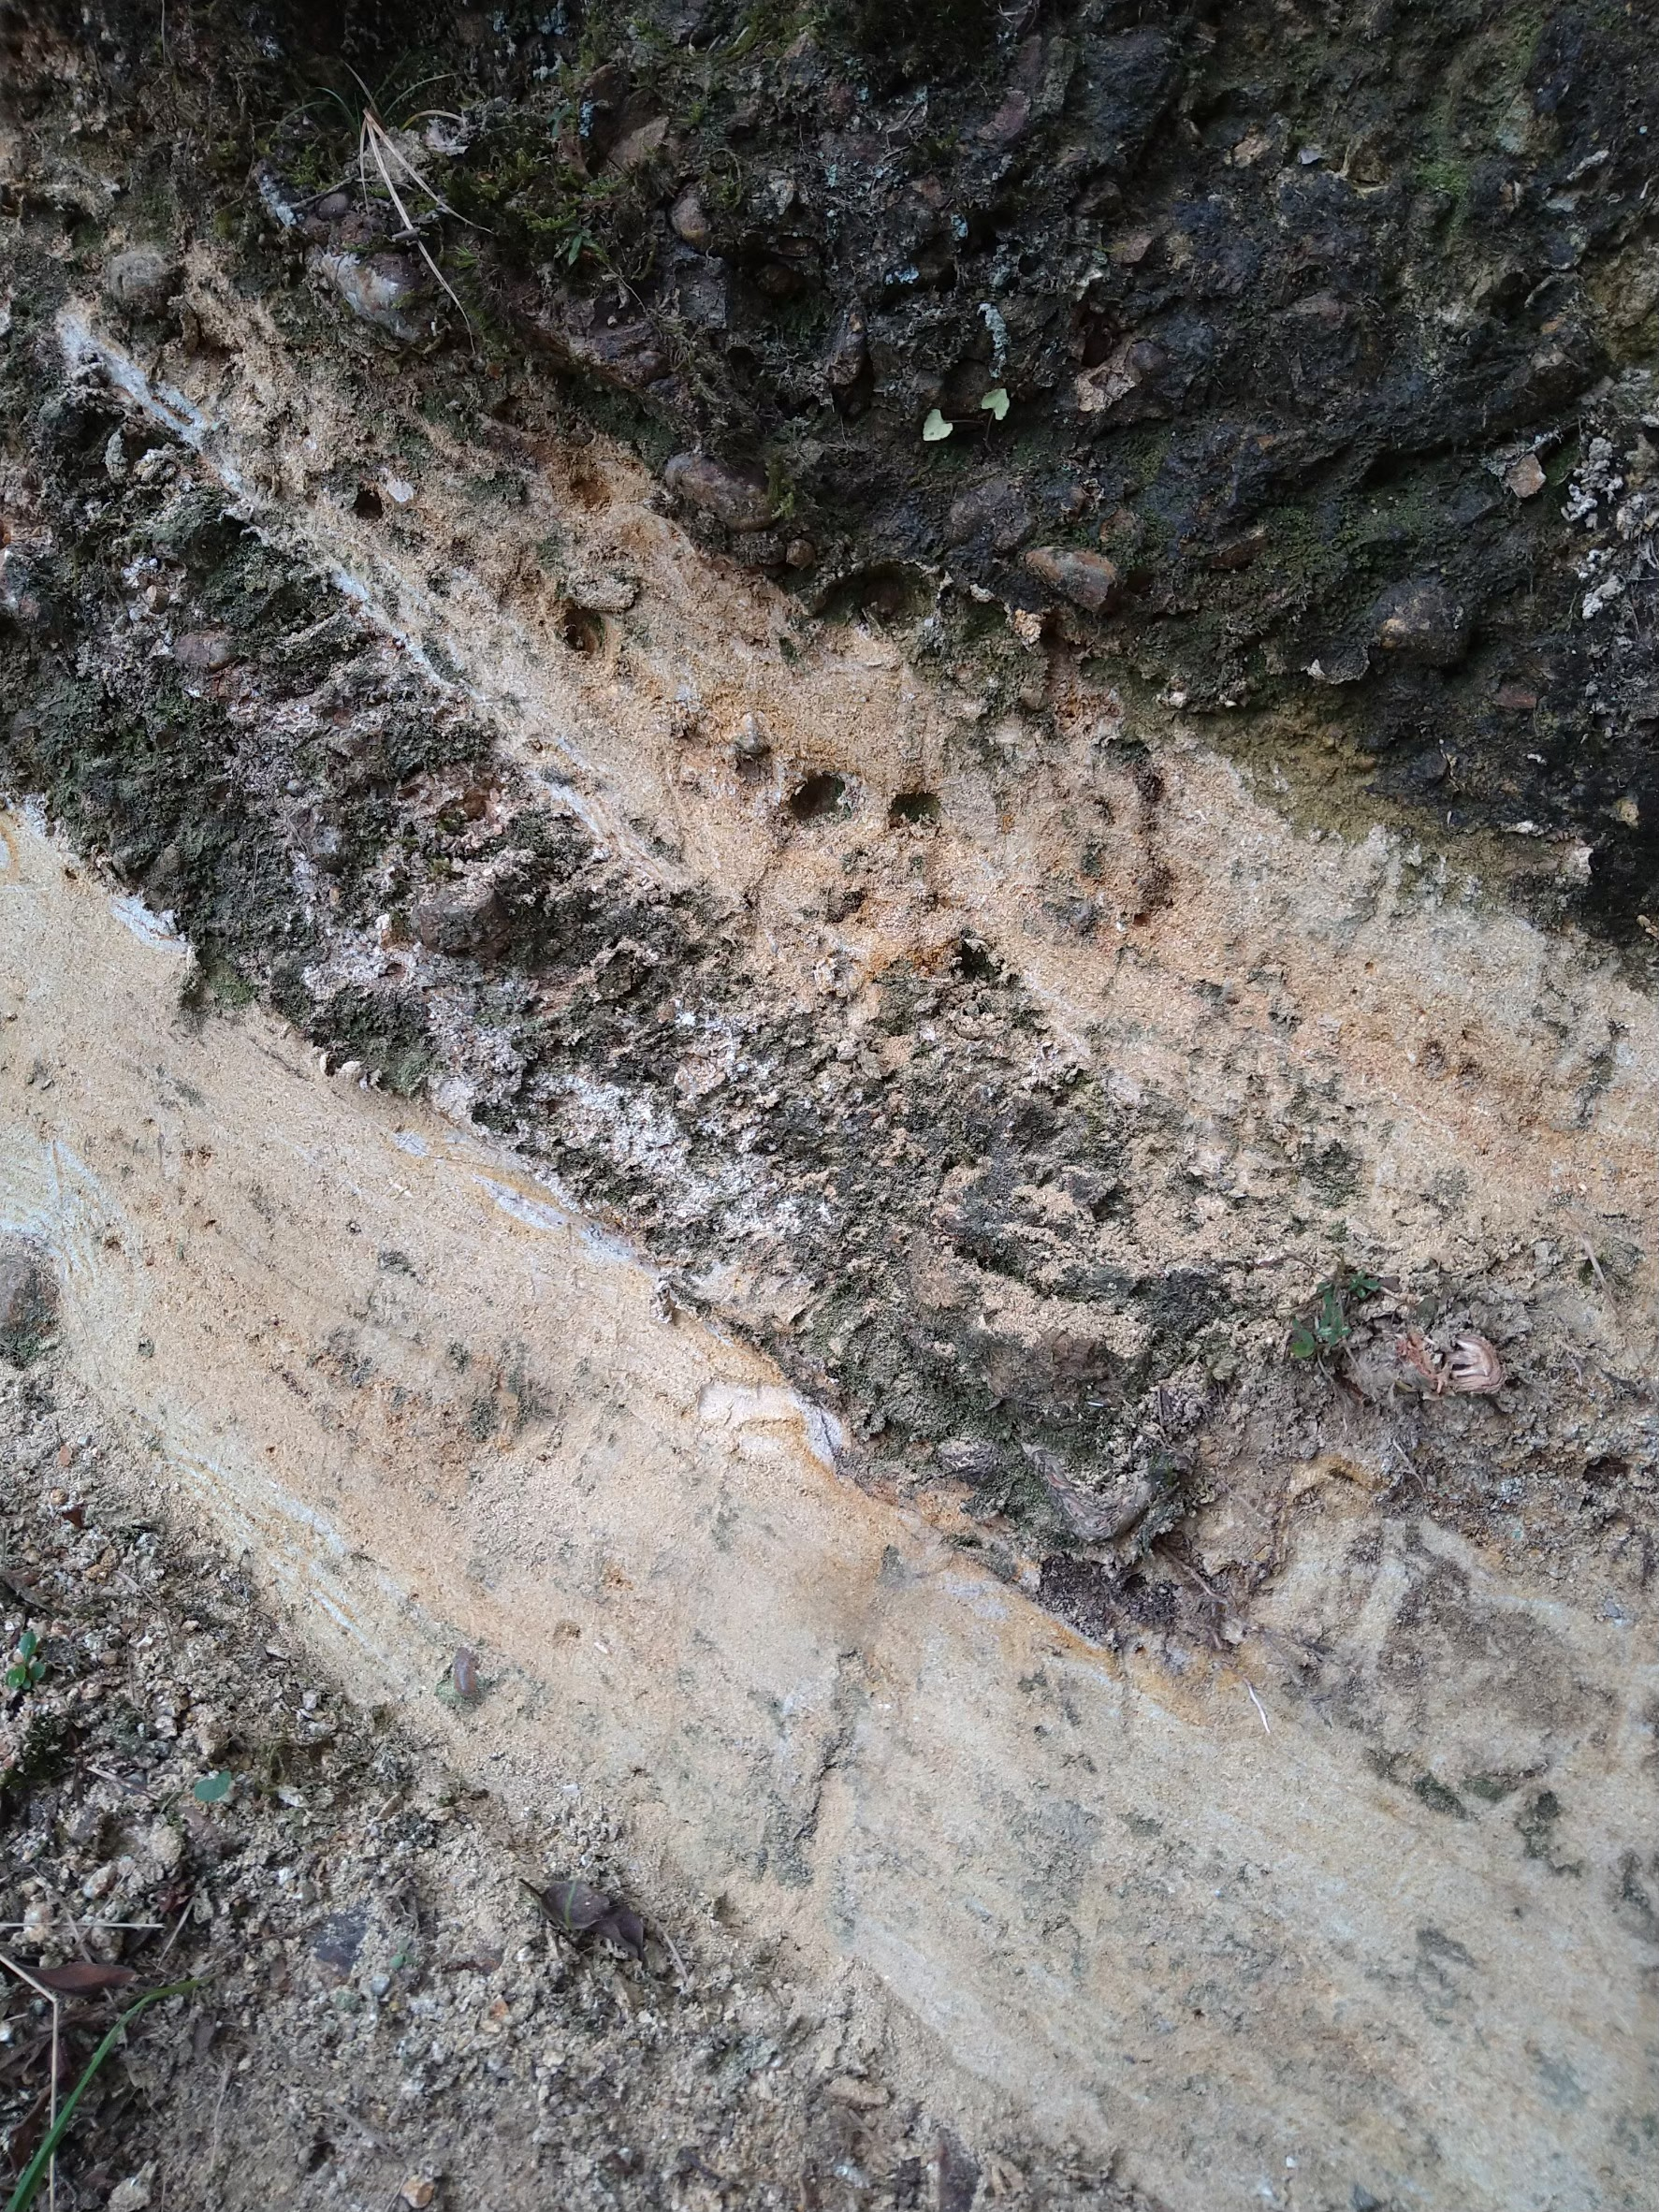
\includegraphics[scale=0.08]{files/地学実習/地点7.jpg}
      \caption{地点7}
    \end{center}    
  \end{figure}
  \clearpage

  \section{地点8}
    \subsection{基本情報}
    岩石:礫岩,シルト岩\par
    走向:EW\par
    特徴:ケスタ地形
    \subsection{設問}
    \leftline{\large \textbf{◎この崖の斜面の走向傾斜を測定し,斜面の構造に注目する。}}
        \paragraph{この斜面は何か。}
        礫岩,シルト岩\footnote{泥岩(\(\frac{1}{16}\)mm以下の大きさの砕屑岩)のうち,\(\frac{1}{256}\)mmより大きいもの。}でできた地形
        \paragraph{少し斜面を上ってみて,特徴的な地形を見つける。}
        ケスタ地形\footnote{「陸上の侵食作用に対して抵抗性が強い硬岩層と,抵抗性が弱い軟岩層とが交互に重なった層(互層)が,侵食されてできた非対称横断面形の起伏をいう。」―コトバンク『ケスタ』}
        \paragraph{どのようにして,このような地形ができたのであろうか?}
        不明
    \subsection{考察}
    直接観察できていないので詳しいことは分からない。
    \begin{figure}[h]
      \begin{center}
        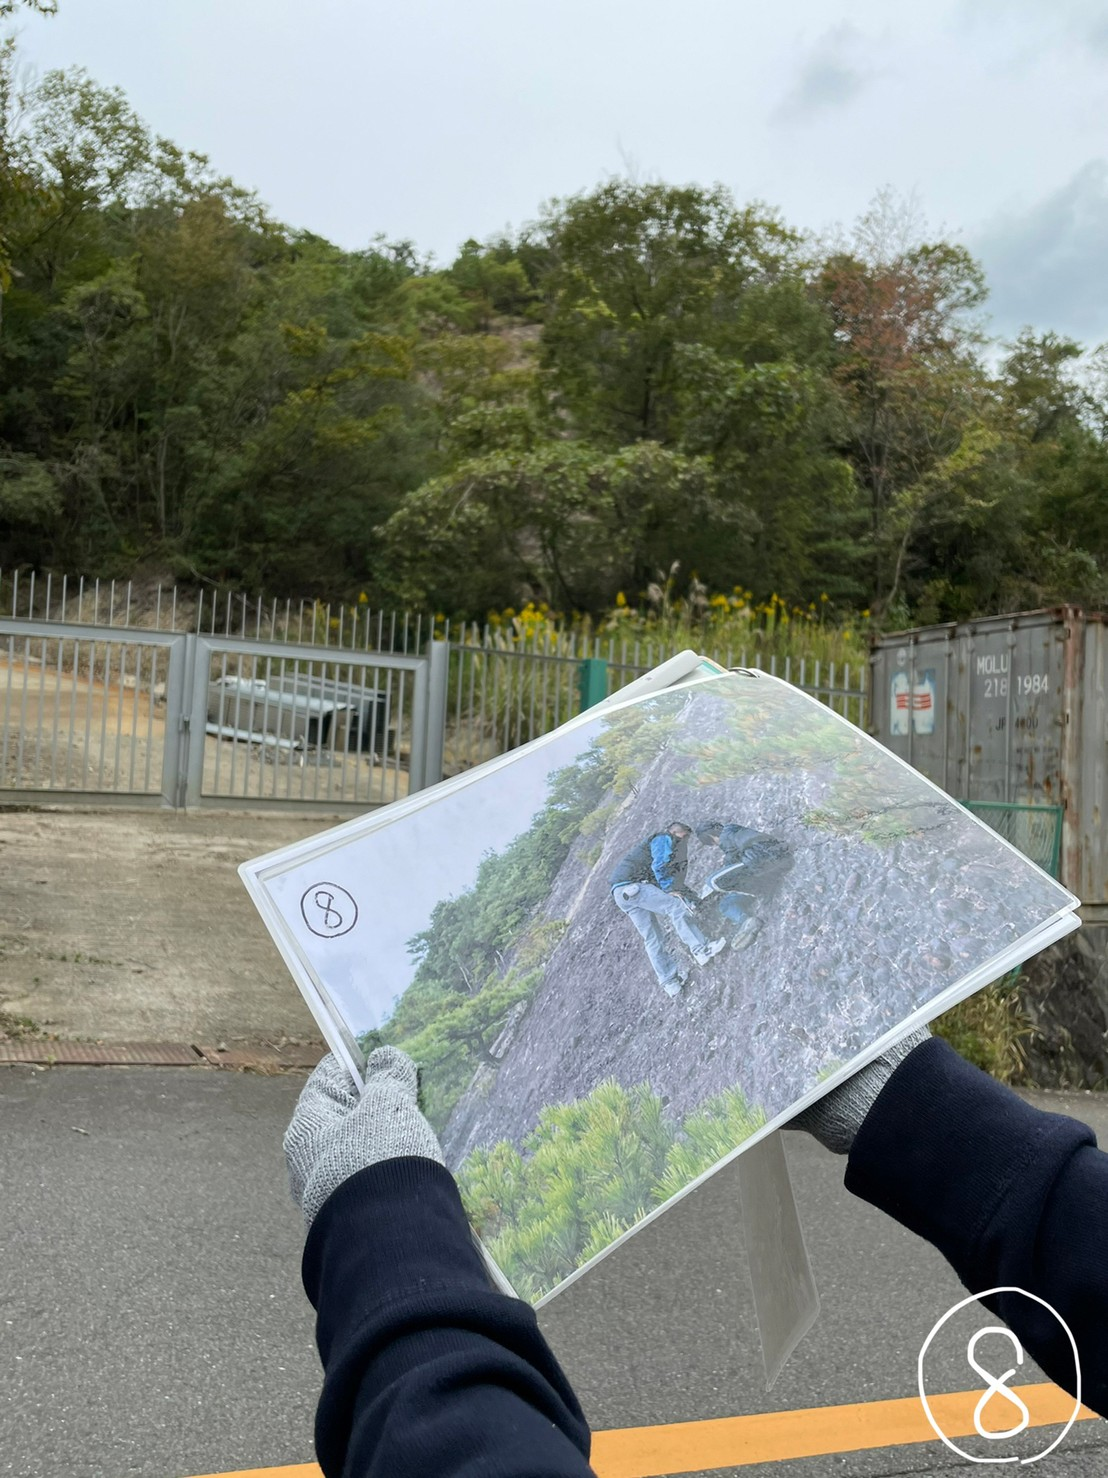
\includegraphics[scale=0.1]{files/地学実習/地点8.jpg}
        \caption{地点8}
      \end{center}    
    \end{figure}
  \clearpage

  \section{地点9}
    \subsection{基本情報}
    岩石:砂岩,火山灰凝灰岩\par
    走向:EW
    \subsection{設問}
    \leftline{\large \textbf{◎露頭を構成する岩石に注目。}}
      \paragraph{今までと様子の違うものはないか?}
      石が簡単に割れる。また,石の粒が細かい。
      \paragraph{色や手触りの違う岩石があれば,手に取って調べてみる。調べた結果,この岩石は何岩といえるか?}
      火山灰凝灰岩
      \paragraph{面が現れていたら,走向傾斜を測定し,地図上に走向線を引いて,これと同じ岩石が他に出る場所があるとすればどこになるか,予想する。}
      向かいの植物のある水辺
      \paragraph{参考として,この層の厚みも測定しておく。}
      70cm
%     \subsection{考察}
  \begin{figure}[h]
    \begin{center}
      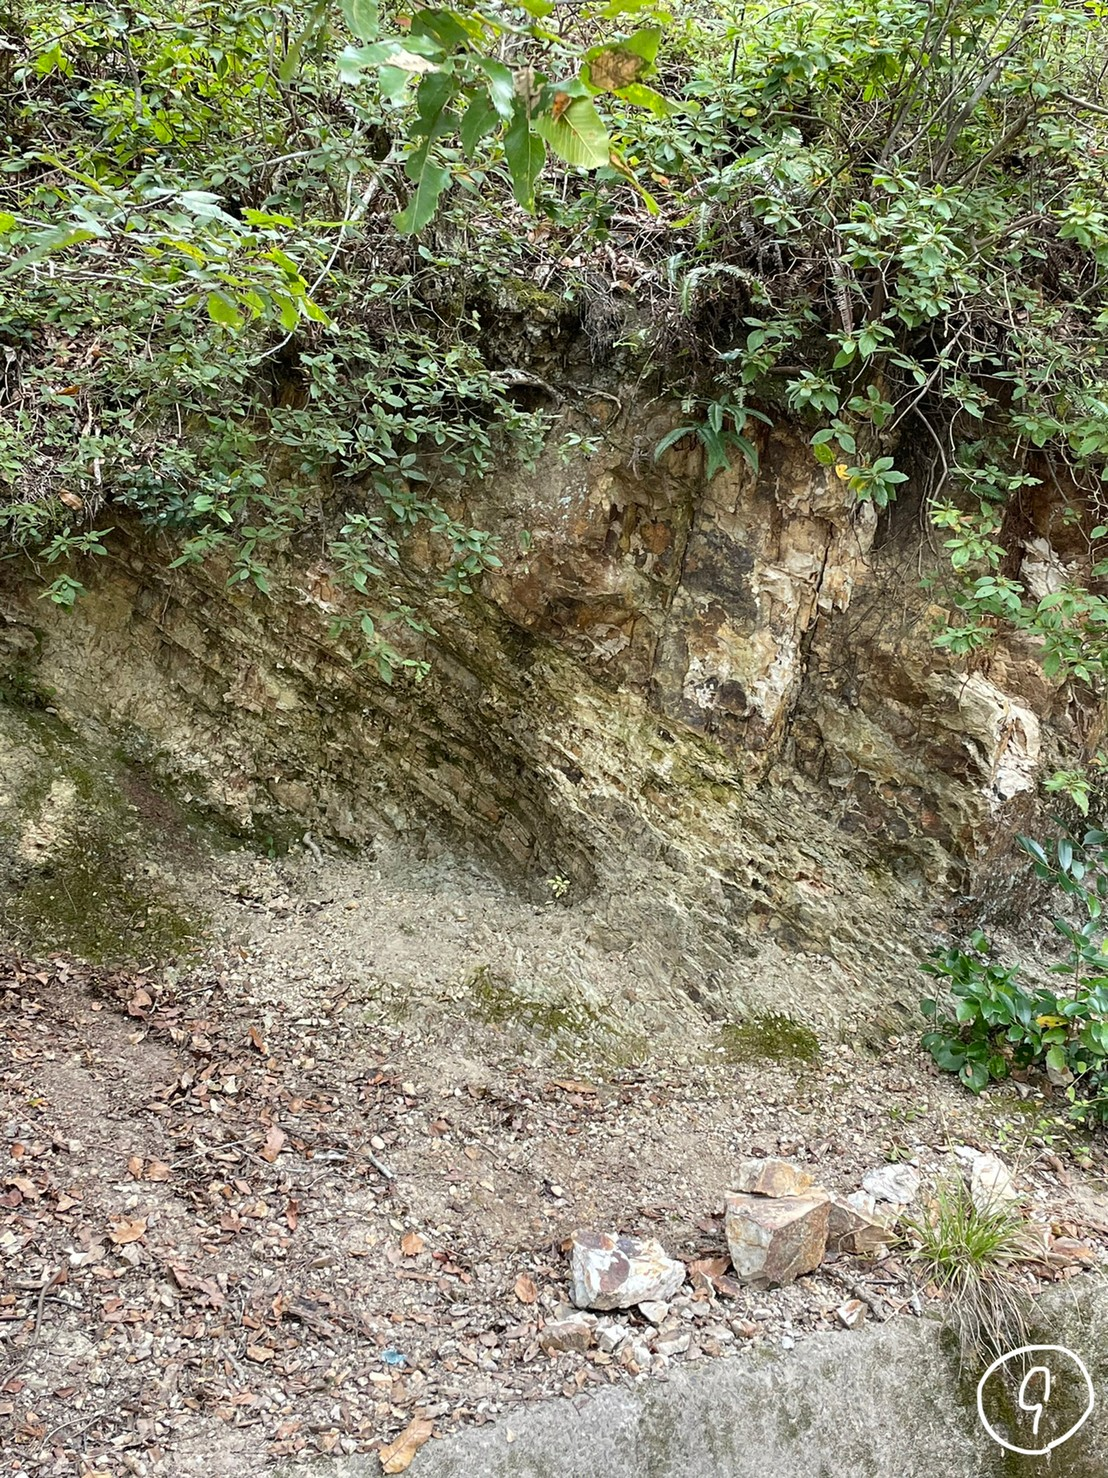
\includegraphics[scale=0.1]{files/地学実習/地点9.jpg}
      \caption{地点9}
    \end{center}    
  \end{figure}
  \clearpage

  \section{地点10}
    \subsection{基本情報}
    岩石:泥岩
    特徴:化石
    \subsection{設問}
    \leftline{\large \textbf{◎露頭を構成している岩石に注目。}}
      \paragraph{この露頭を構成する岩石は何か?また,どのような環境でできたと考えられるか?}
      泥岩。海の深いところ。
      \paragraph{足元に転がっている石を拾ってみて,化石が含まれていないか確かめる。ハンマーで叩いて割っているのもよい。ただし,柵の向こう側には入らないこと。この地層からはどのような化石が出てくるのだろうか。}
      化石は得られなかったが,海に生息する生物の化石が出てくると考えられる。
      \paragraph{化石から判断して,この地層はどのような環境のもと,今からどれぐらい前にできたと考えられるか?}
      化石が得られなかったので詳しいことは判断できない。
    \subsection{考察}
    同上
  \begin{figure}[h]
    \begin{center}
      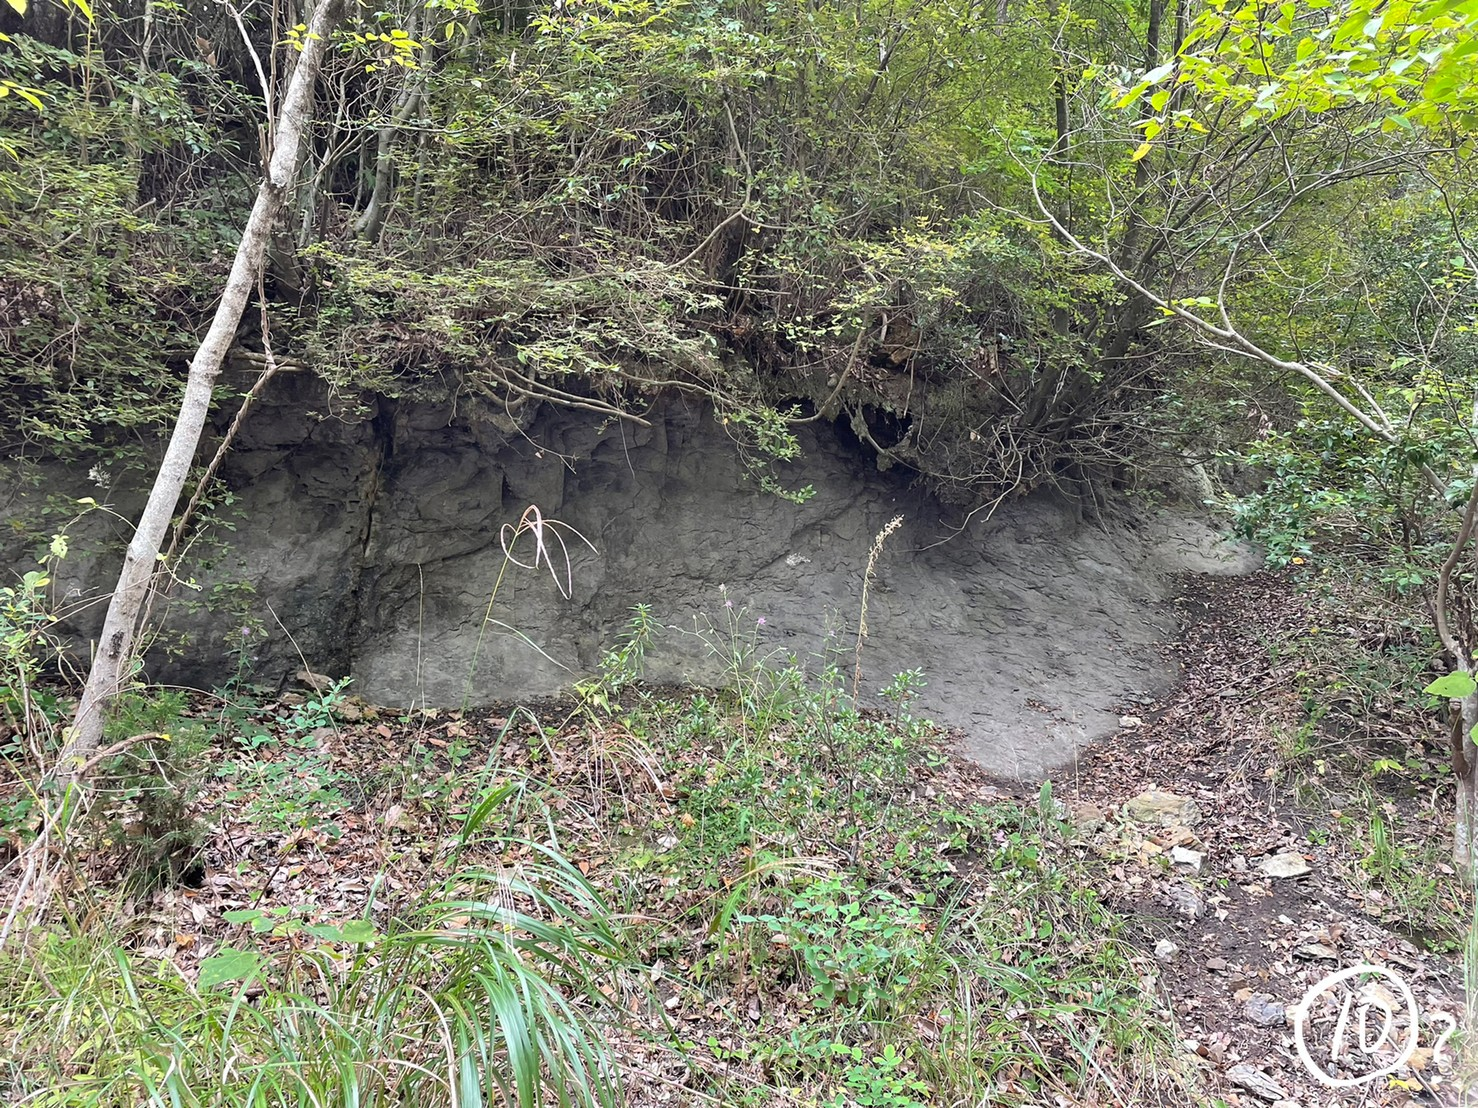
\includegraphics[scale=0.13]{files/地学実習/地点10.jpg}
      \caption{地点10}
    \end{center}    
  \end{figure}
  \clearpage

  \section{地点11}
    \subsection{基本情報}
    基本情報:砂岩,凝灰岩\par
    走向:N60\textdegree W
    \subsection{設問}
    \leftline{\large \textbf{◎ブロックの上の崖に注目。}}
      \paragraph{どのような岩石が見られるか?}
      砂岩と凝灰岩の層ができている。
      \paragraph{出ている地層面の走向傾斜を測定する。何か気付くことはないか?}
      川の向きと同じ向きになっている。
    \subsection{考察}
    複数層あることからも,また走向と川の向きが近しいことからもこの地層は過去に川底\footnote{海底の可能性も当然あるが,近くに河岸段丘が見られることも踏まえて川底とした。}であったと考えられる。
  \clearpage

  \section{地点12}
    \subsection{基本情報}
    岩石:礫岩
    \subsection{設問}
    \leftline{\large \textbf{◎露頭を構成する岩石に注目。}}
      \paragraph{礫の大きさ(最大径),形,礫種を調べる。なぜこのような礫が現れるのだろうか?地図上で位置を確かめ,これまで見てきたことから考える。}
      大きめで約100mm(大礫)。地点5の礫と同じであり,和泉群層のものと思われる。
      \paragraph{この地点から,次の地点までの間に,礫の様子はどのように変化していくか予想してみる。}
      大きくなっていく。
    \subsection{考察}
    和泉群層が現れたということは,より北上すれば泉南流紋岩が現れ始めると考えられる。
  \begin{figure}[h]
    \begin{center}
      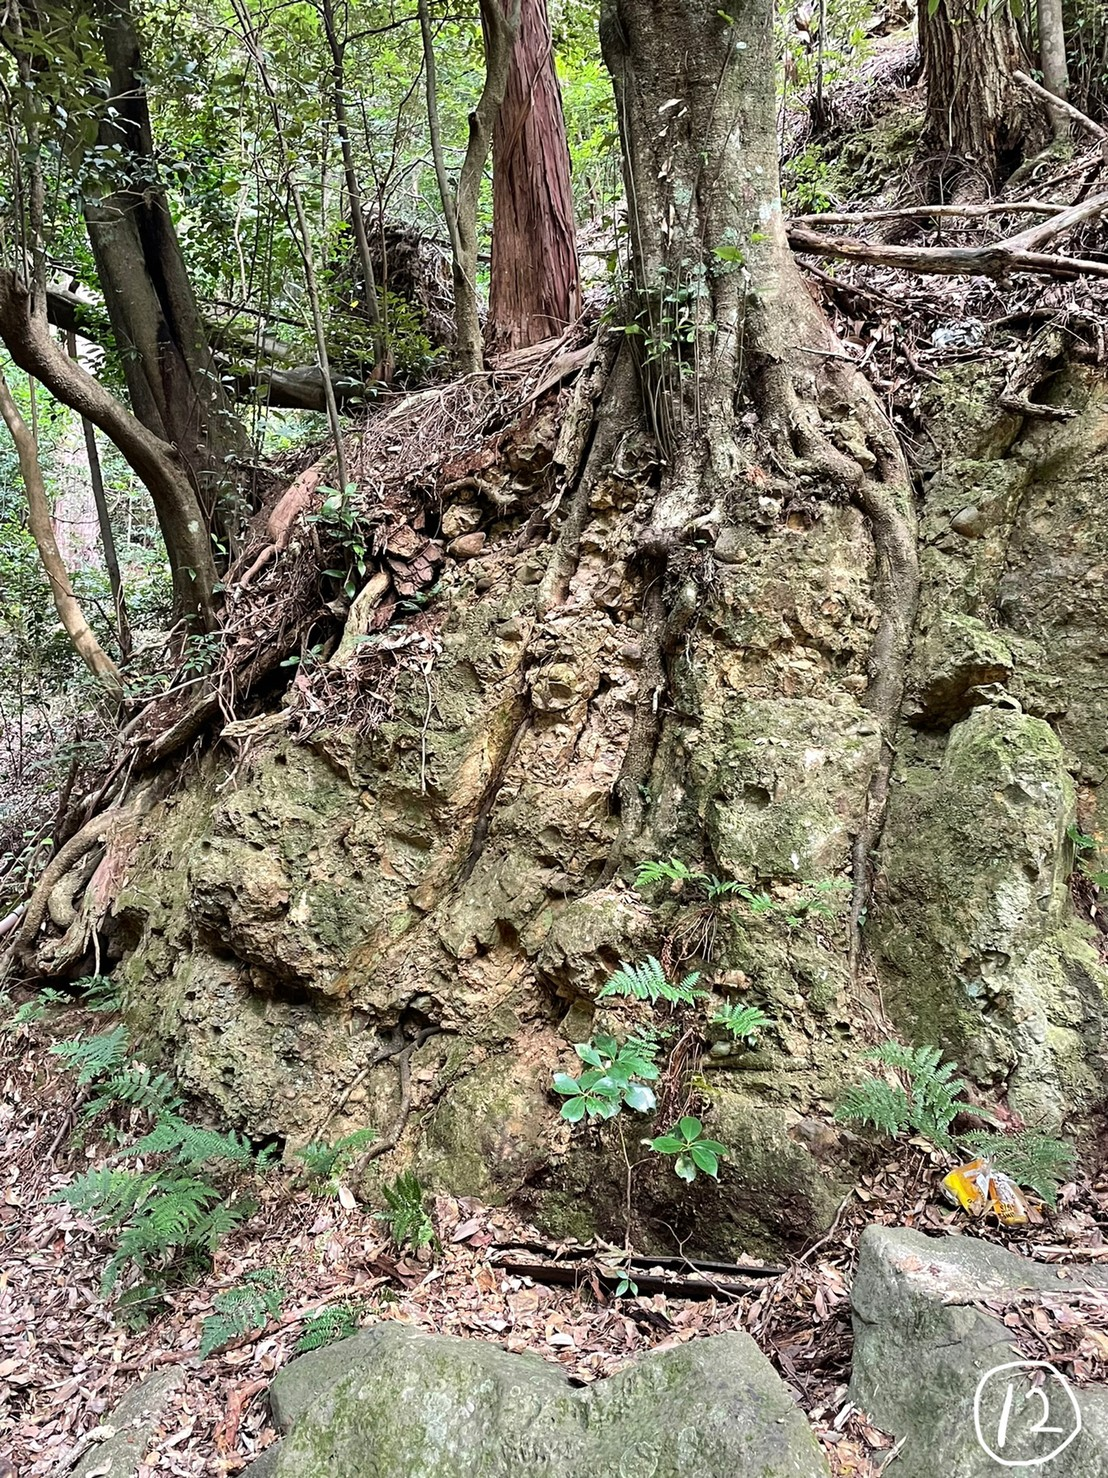
\includegraphics[scale=0.15]{files/地学実習/地点12.jpg}
      \caption{地点12}
    \end{center}    
  \end{figure}
  \clearpage

  \section{地点13}
    \subsection{基本情報}
    岩石:礫
    \subsection{設問}
    \leftline{\large \textbf{◎礫の大きさに注目。予想どおりか?}}
    地点12よりも大きくなっている(予想どおり。)。
%     \subsection{考察}
  \begin{figure}[h]
    \begin{center}
      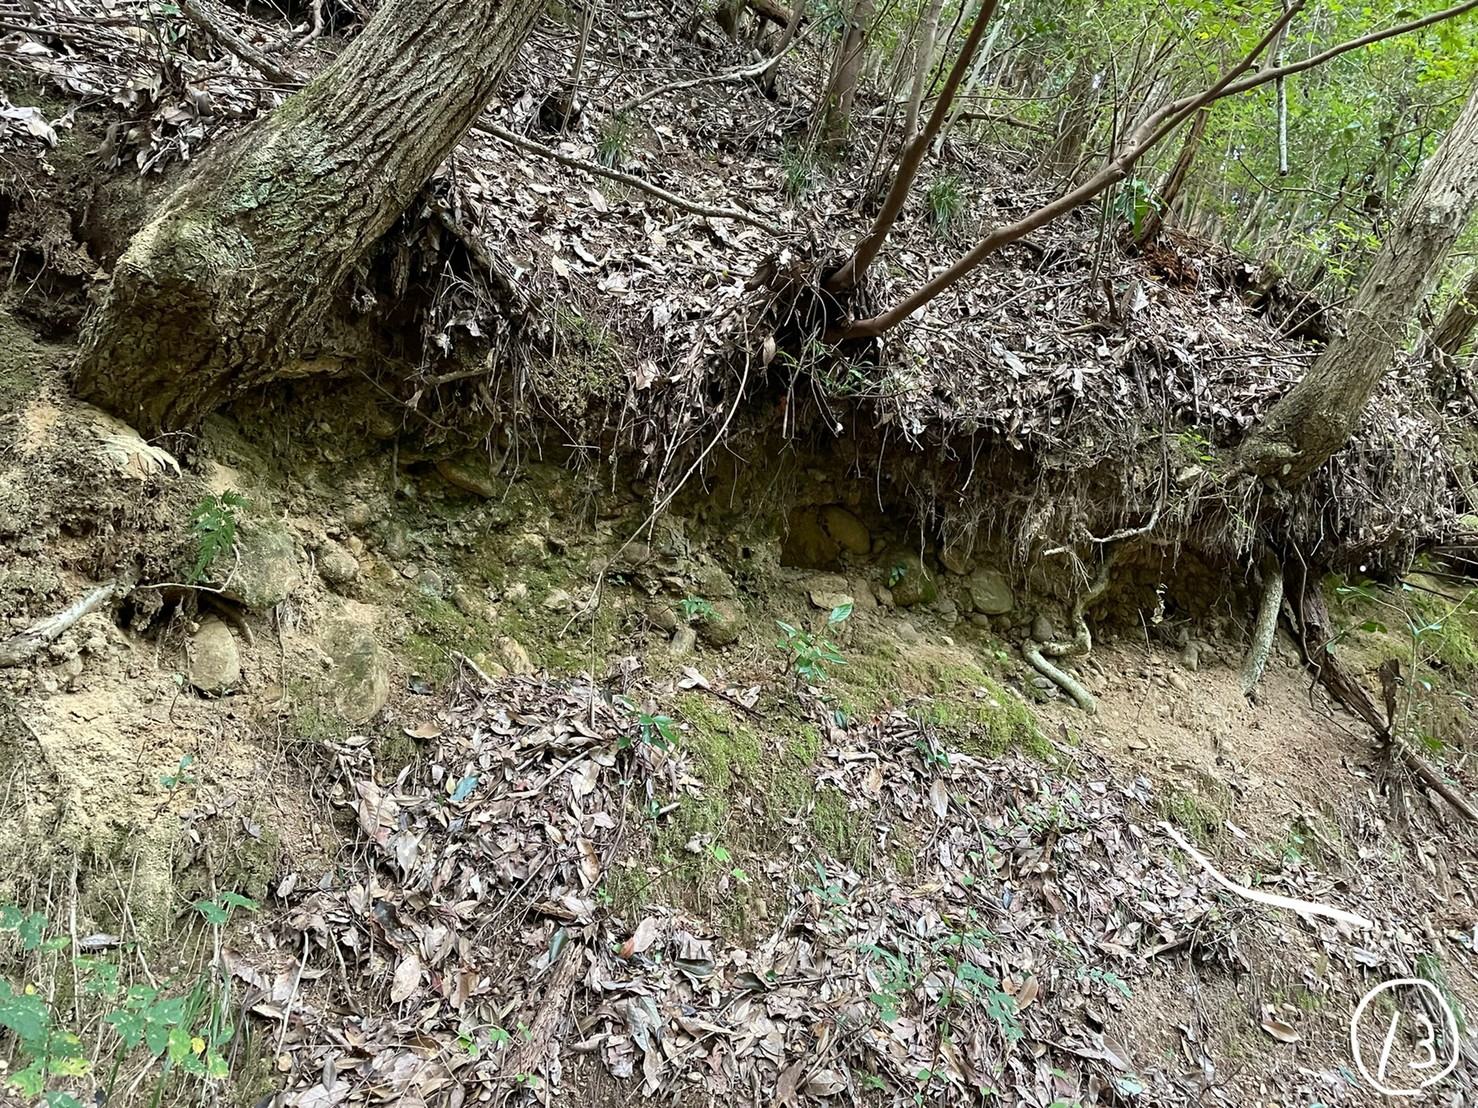
\includegraphics[scale=0.25]{files/地学実習/地点13.jpg}
      \caption{地点13}
    \end{center}    
  \end{figure}
  \clearpage

  \section{地点14}
    \subsection{基本情報}
    岩石:礫岩,泉南流紋岩\par
    走向:N20\textdegree W
    \subsection{設問}
    \leftline{\large \textbf{◎谷の奥に注目。}}
      \paragraph{どのような岩石が見られるか?}
      礫岩,泉南流紋岩
      \paragraph{今までに見てきた露頭と比較してみる。様子が似ている地点はなかったか?また地図上でのその位置を確かめる。}
      地点5に近い。
%     \subsection{考察}
  \begin{figure}[h]
    \begin{center}
      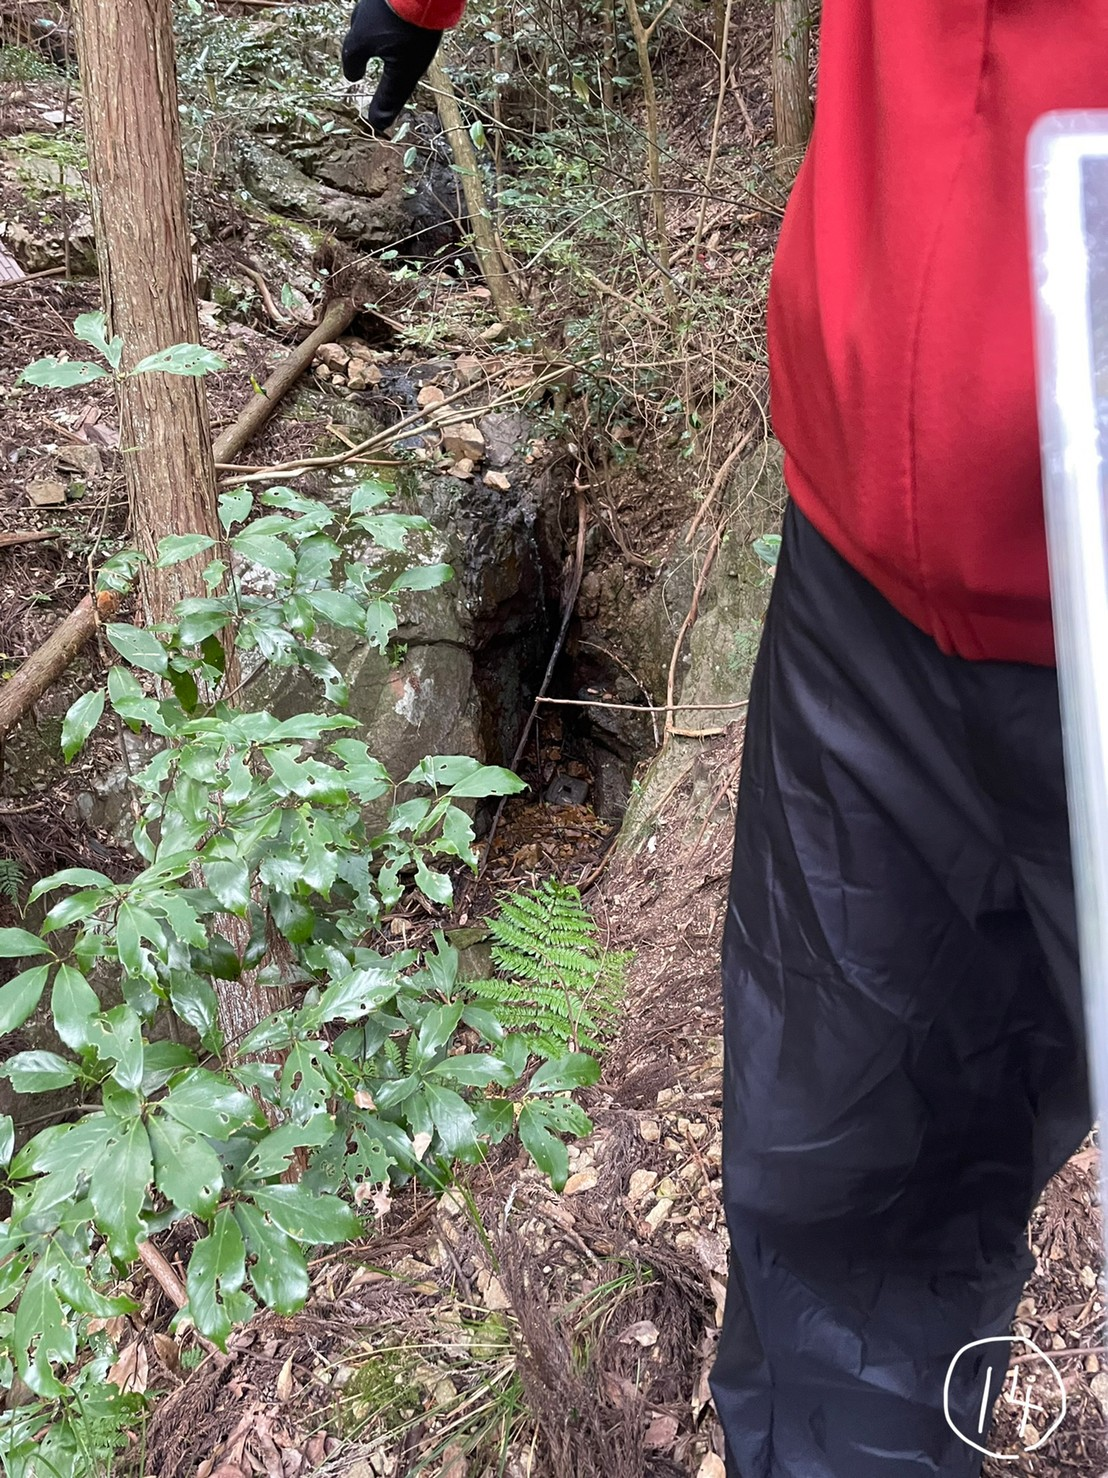
\includegraphics[scale=0.15]{files/地学実習/地点14.jpg}
      \caption{地点14}
    \end{center}    
  \end{figure}
  \clearpage

  \section{地点15}
    \subsection{基本情報}
    岩石:礫岩,砂岩\par
    走向:EW\par
    傾斜:60\textdegree S
    \subsection{設問}
    \leftline{\large \textbf{◎露頭を構成する地層の傾き具合に注目。}}
      \paragraph{補助版を当てて,走向傾斜を測定する。}
      補助版での測定なので誤差が大きいことが予想されるのが懸念事項である。
%     \subsection{考察}
  \begin{figure}[h]
    \begin{center}
      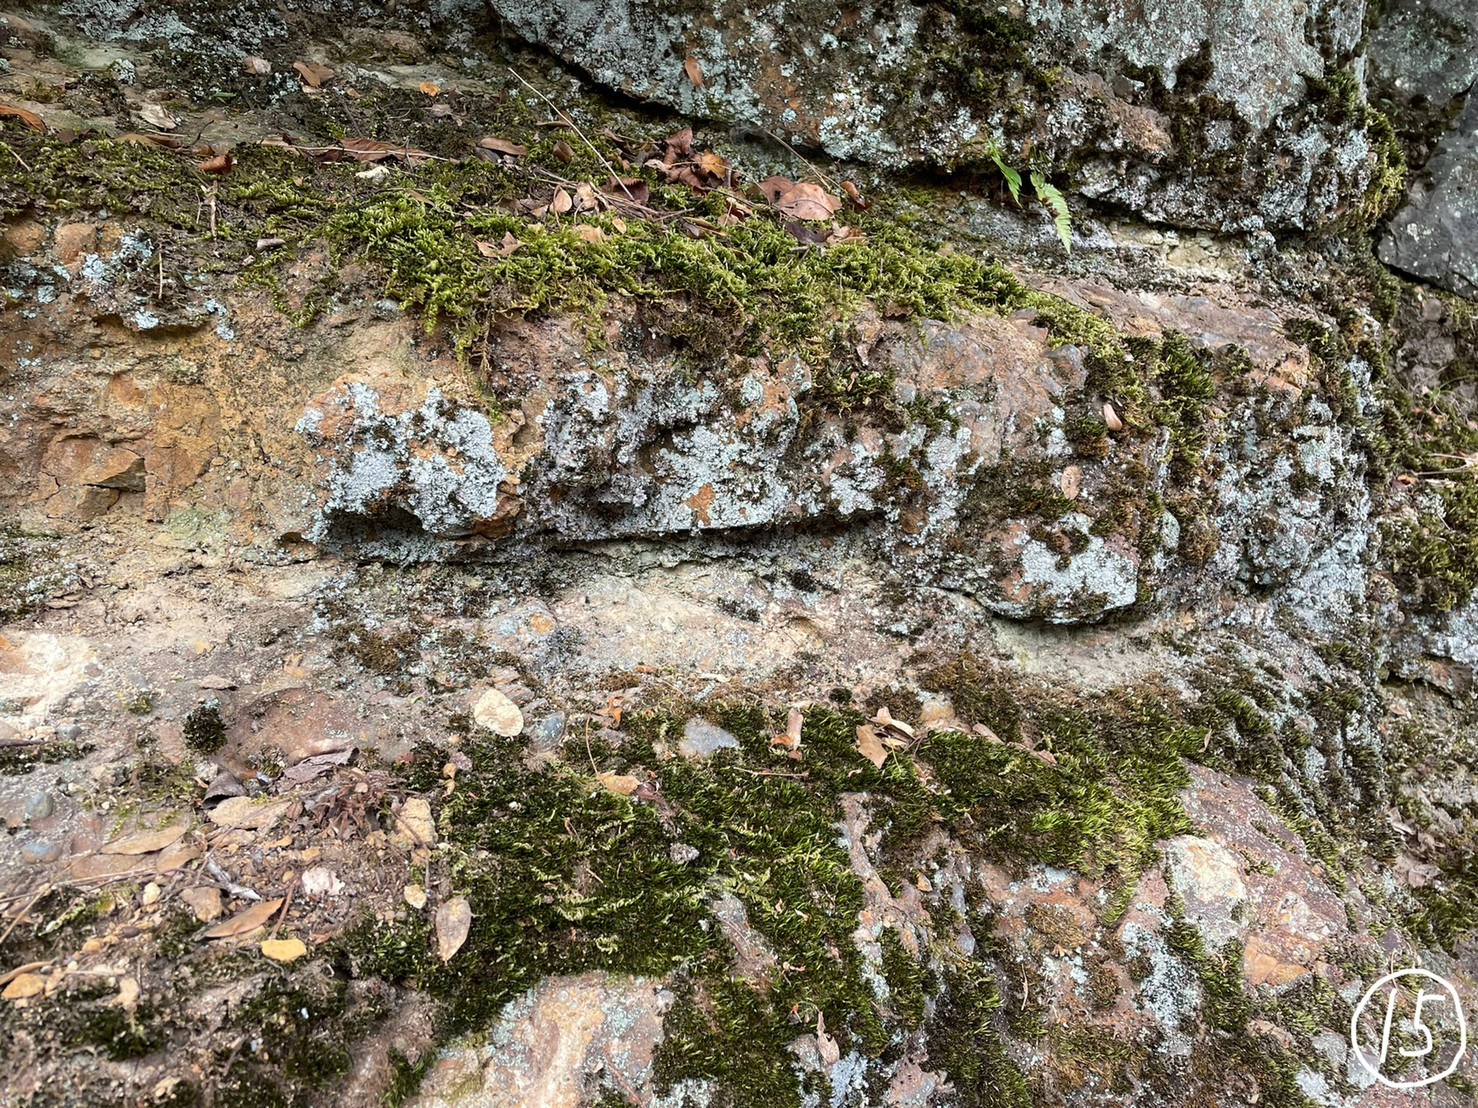
\includegraphics[scale=0.1]{files/地学実習/地点15_1.jpg}
      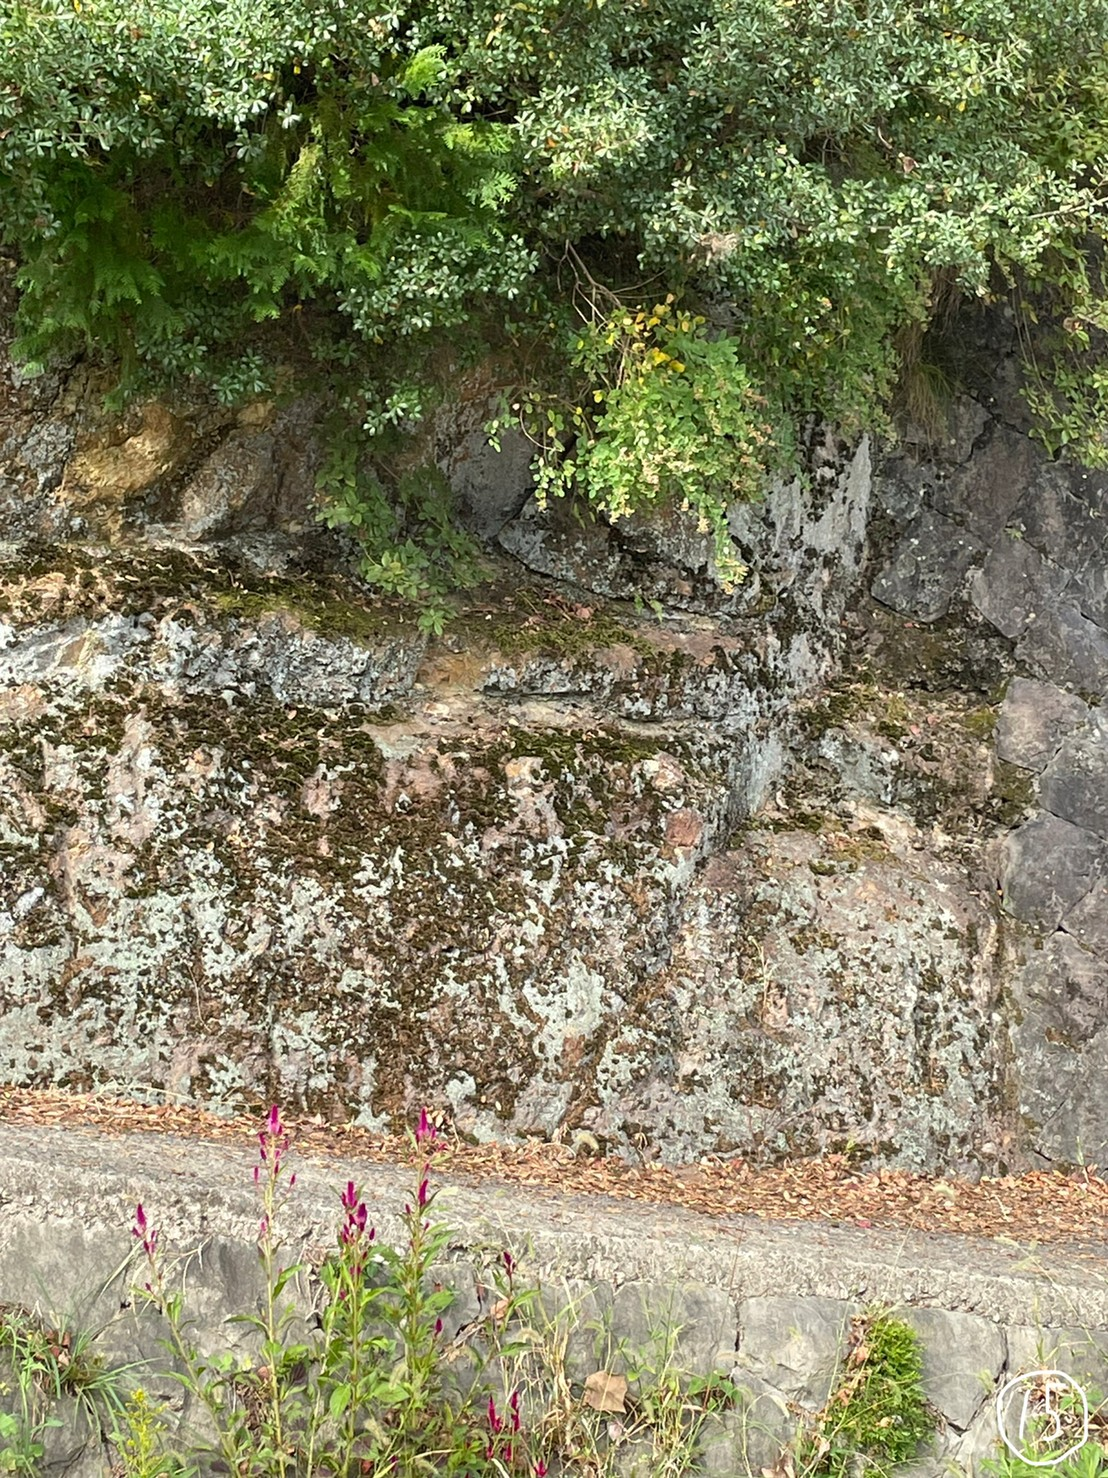
\includegraphics[scale=0.15]{files/地学実習/地点15_2.jpg}
      \caption{地点15}
    \end{center}
  \end{figure}
  \clearpage

  \section{地点16}
    \subsection{基本情報}
    特徴:河岸段丘
    \subsection{設問}
    \leftline{\large \textbf{◎橋の上から,田圃の景色を眺めてみる。}}
      \paragraph{この地形は何か?}
      北側に河岸段丘,南側に崖がある。
      \paragraph{平坦な面は何段ぐらいあるか。またそれらはどのような地盤の運動で生じたか。}
      5段ほど。河岸段丘は地盤の隆起や海退によって引き起こる(図表p.129)。
    \subsection{考察}
    この川よりも高い位置にある地層にも隆起や海退によってできる互層が見られることから,遥か昔は海底にあり,それが隆起して川ができたのちに更に隆起や海退が起こったことによってこのような地形ができたと考えられる。
  \begin{figure}[h]
    \begin{center}
      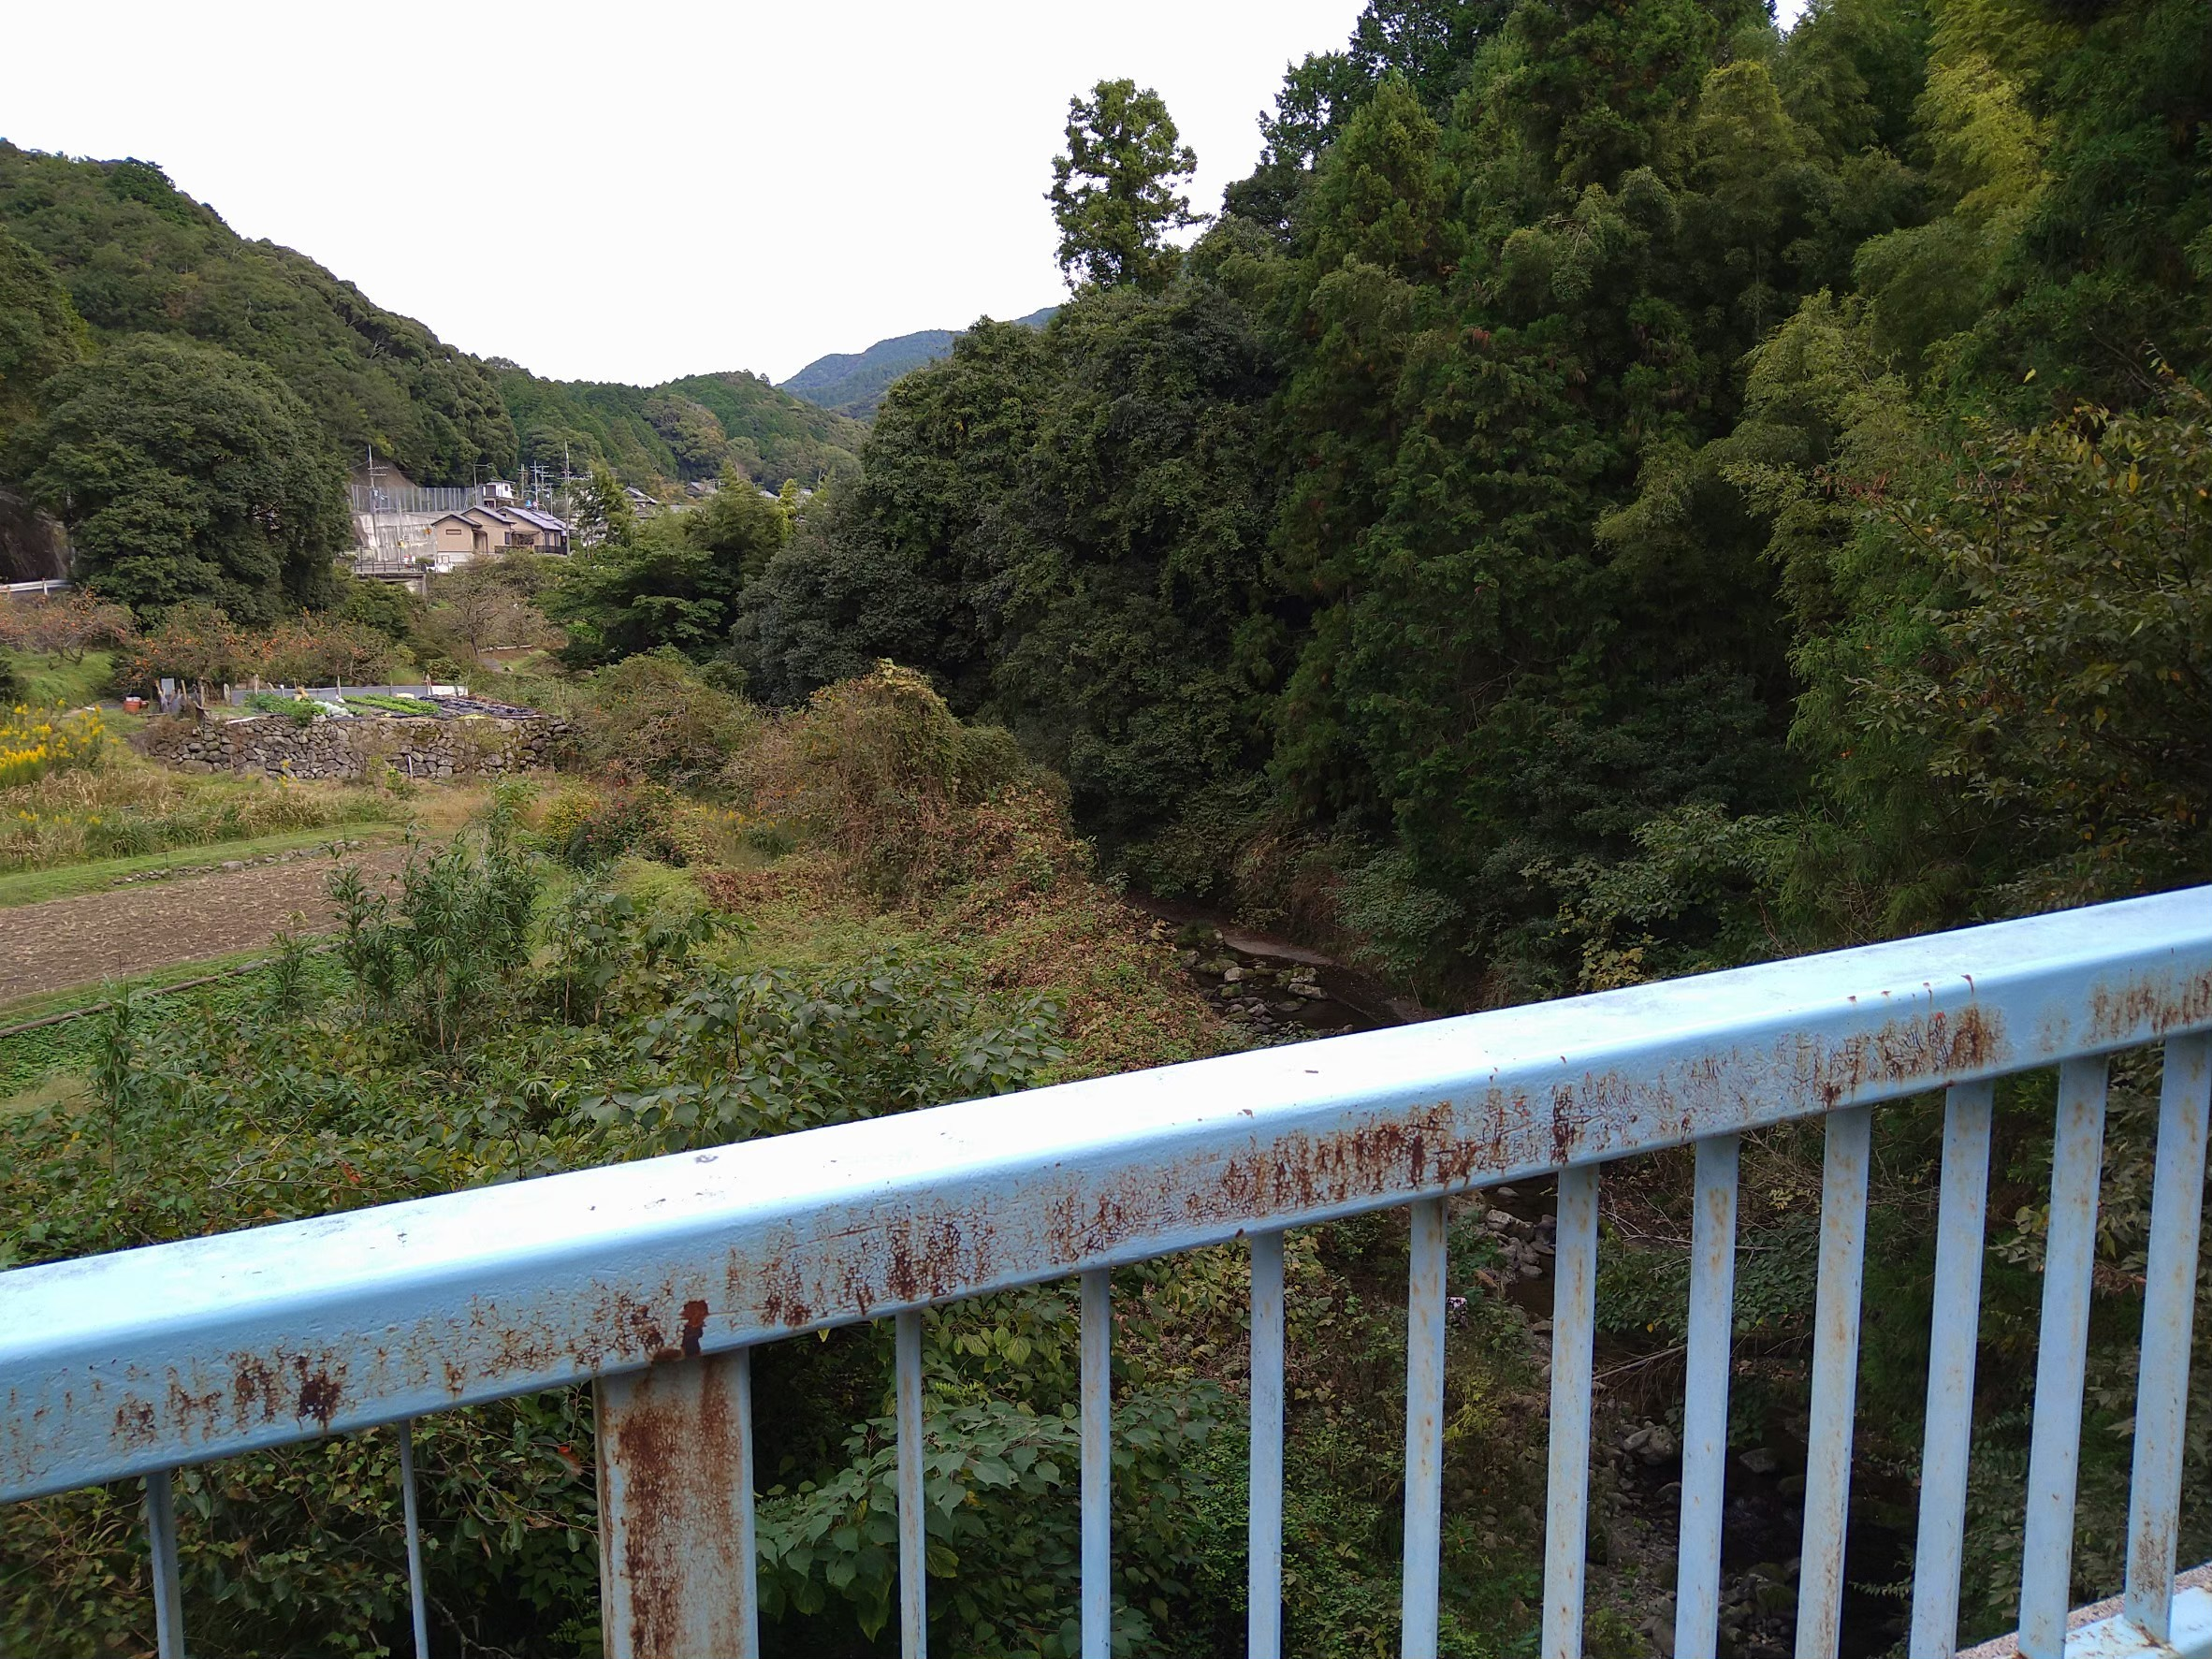
\includegraphics[scale=0.12]{files/地学実習/地点16.jpg}
      \caption{地点16}
    \end{center}
  \end{figure}
  \clearpage

  \section{地点17}
    \subsection{基本情報}
    岩石:礫岩,泉南流紋岩
    特徴:秋山不整合
    \subsection{設問}
    \leftline{\large \textbf{◎河床に見られる岩石(転がっているものではなく,下の岩体を構成するもの))}}
      \paragraph{場所によって何か変化はないか?ここには地学上ののどのような構造が見られるのだろうか?}
      北に向かうにつれて,とても大きな礫岩から泉南流紋岩へ地層が変化している(不整合面)。
    \subsection{考察}
    地点5で見られたように,和泉層群と泉南流紋岩の境目である秋山不整合がここにも現れている。
  \begin{figure}[h]
    \begin{center}
      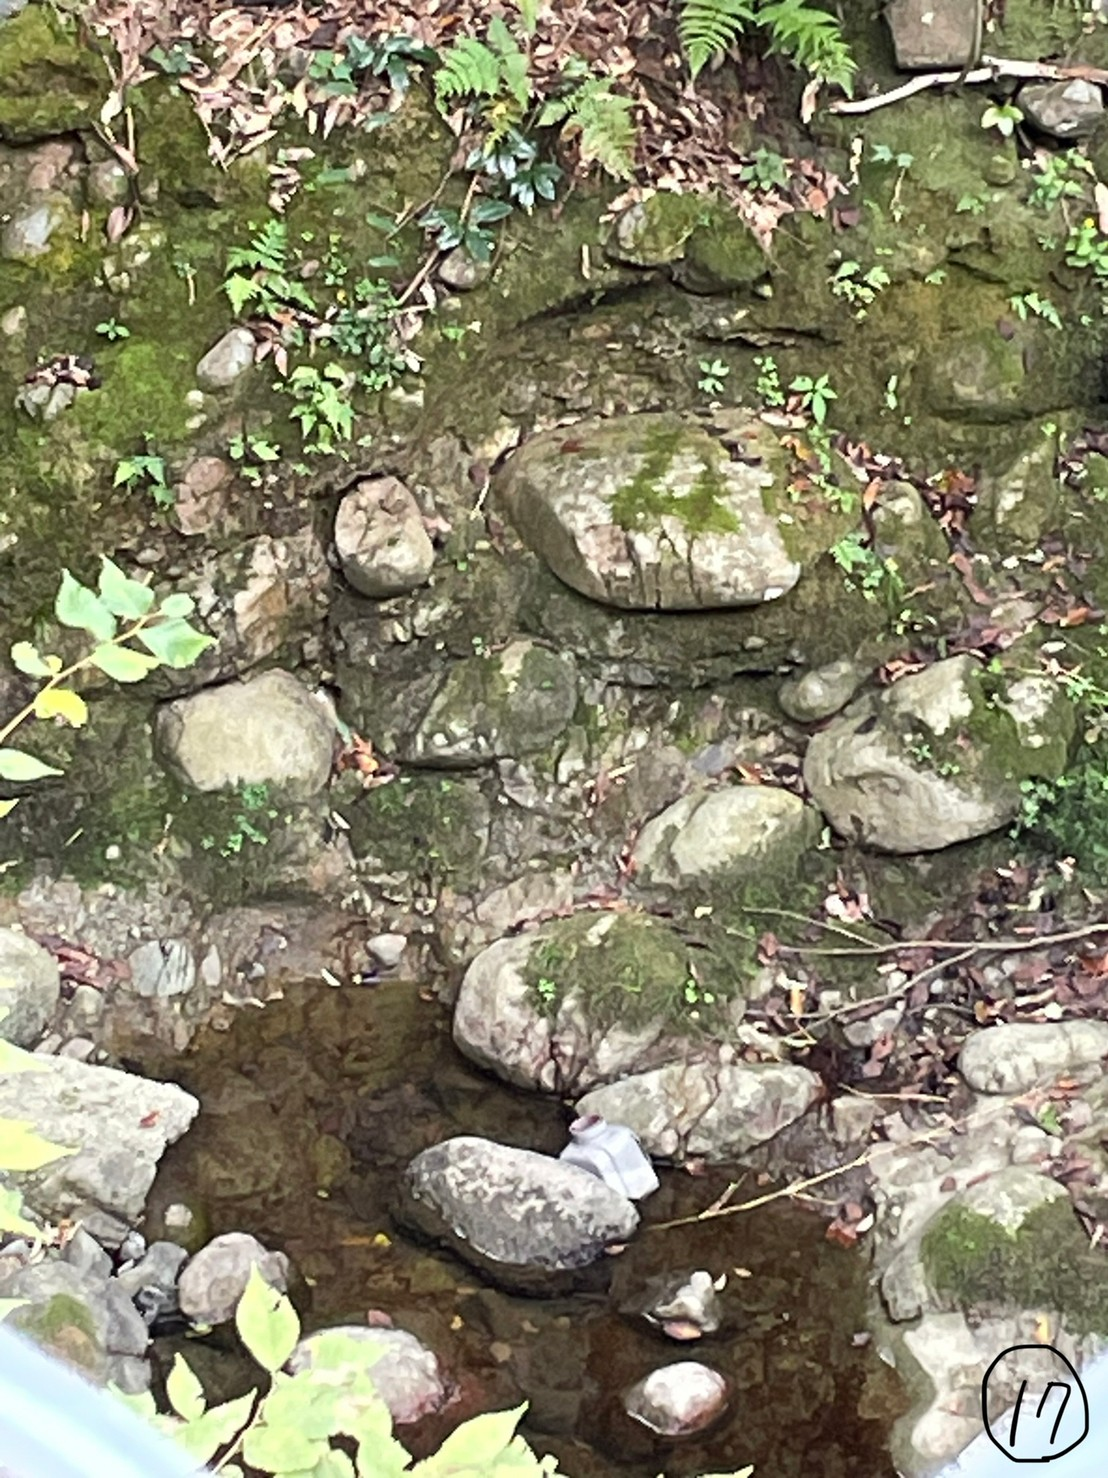
\includegraphics[scale=0.15]{files/地学実習/地点17.jpg}
      \caption{地点17}
    \end{center}    
  \end{figure}
  \clearpage

  \section{地点18}
    \subsection{基本情報}
    岩石:礫岩
    \subsection{設問}
    \leftline{\large \textbf{◎奥水園霊園の大きな崖に注目。}}
      \paragraph{これまで見てきたことから判断して,ここにどのような構造が見られるのか予想する。そしてそれはどこに見られるか。}
      礫岩と泉南流紋岩の不整合面。
%     \subsection{考察}
  \begin{figure}[h]
    \begin{center}
      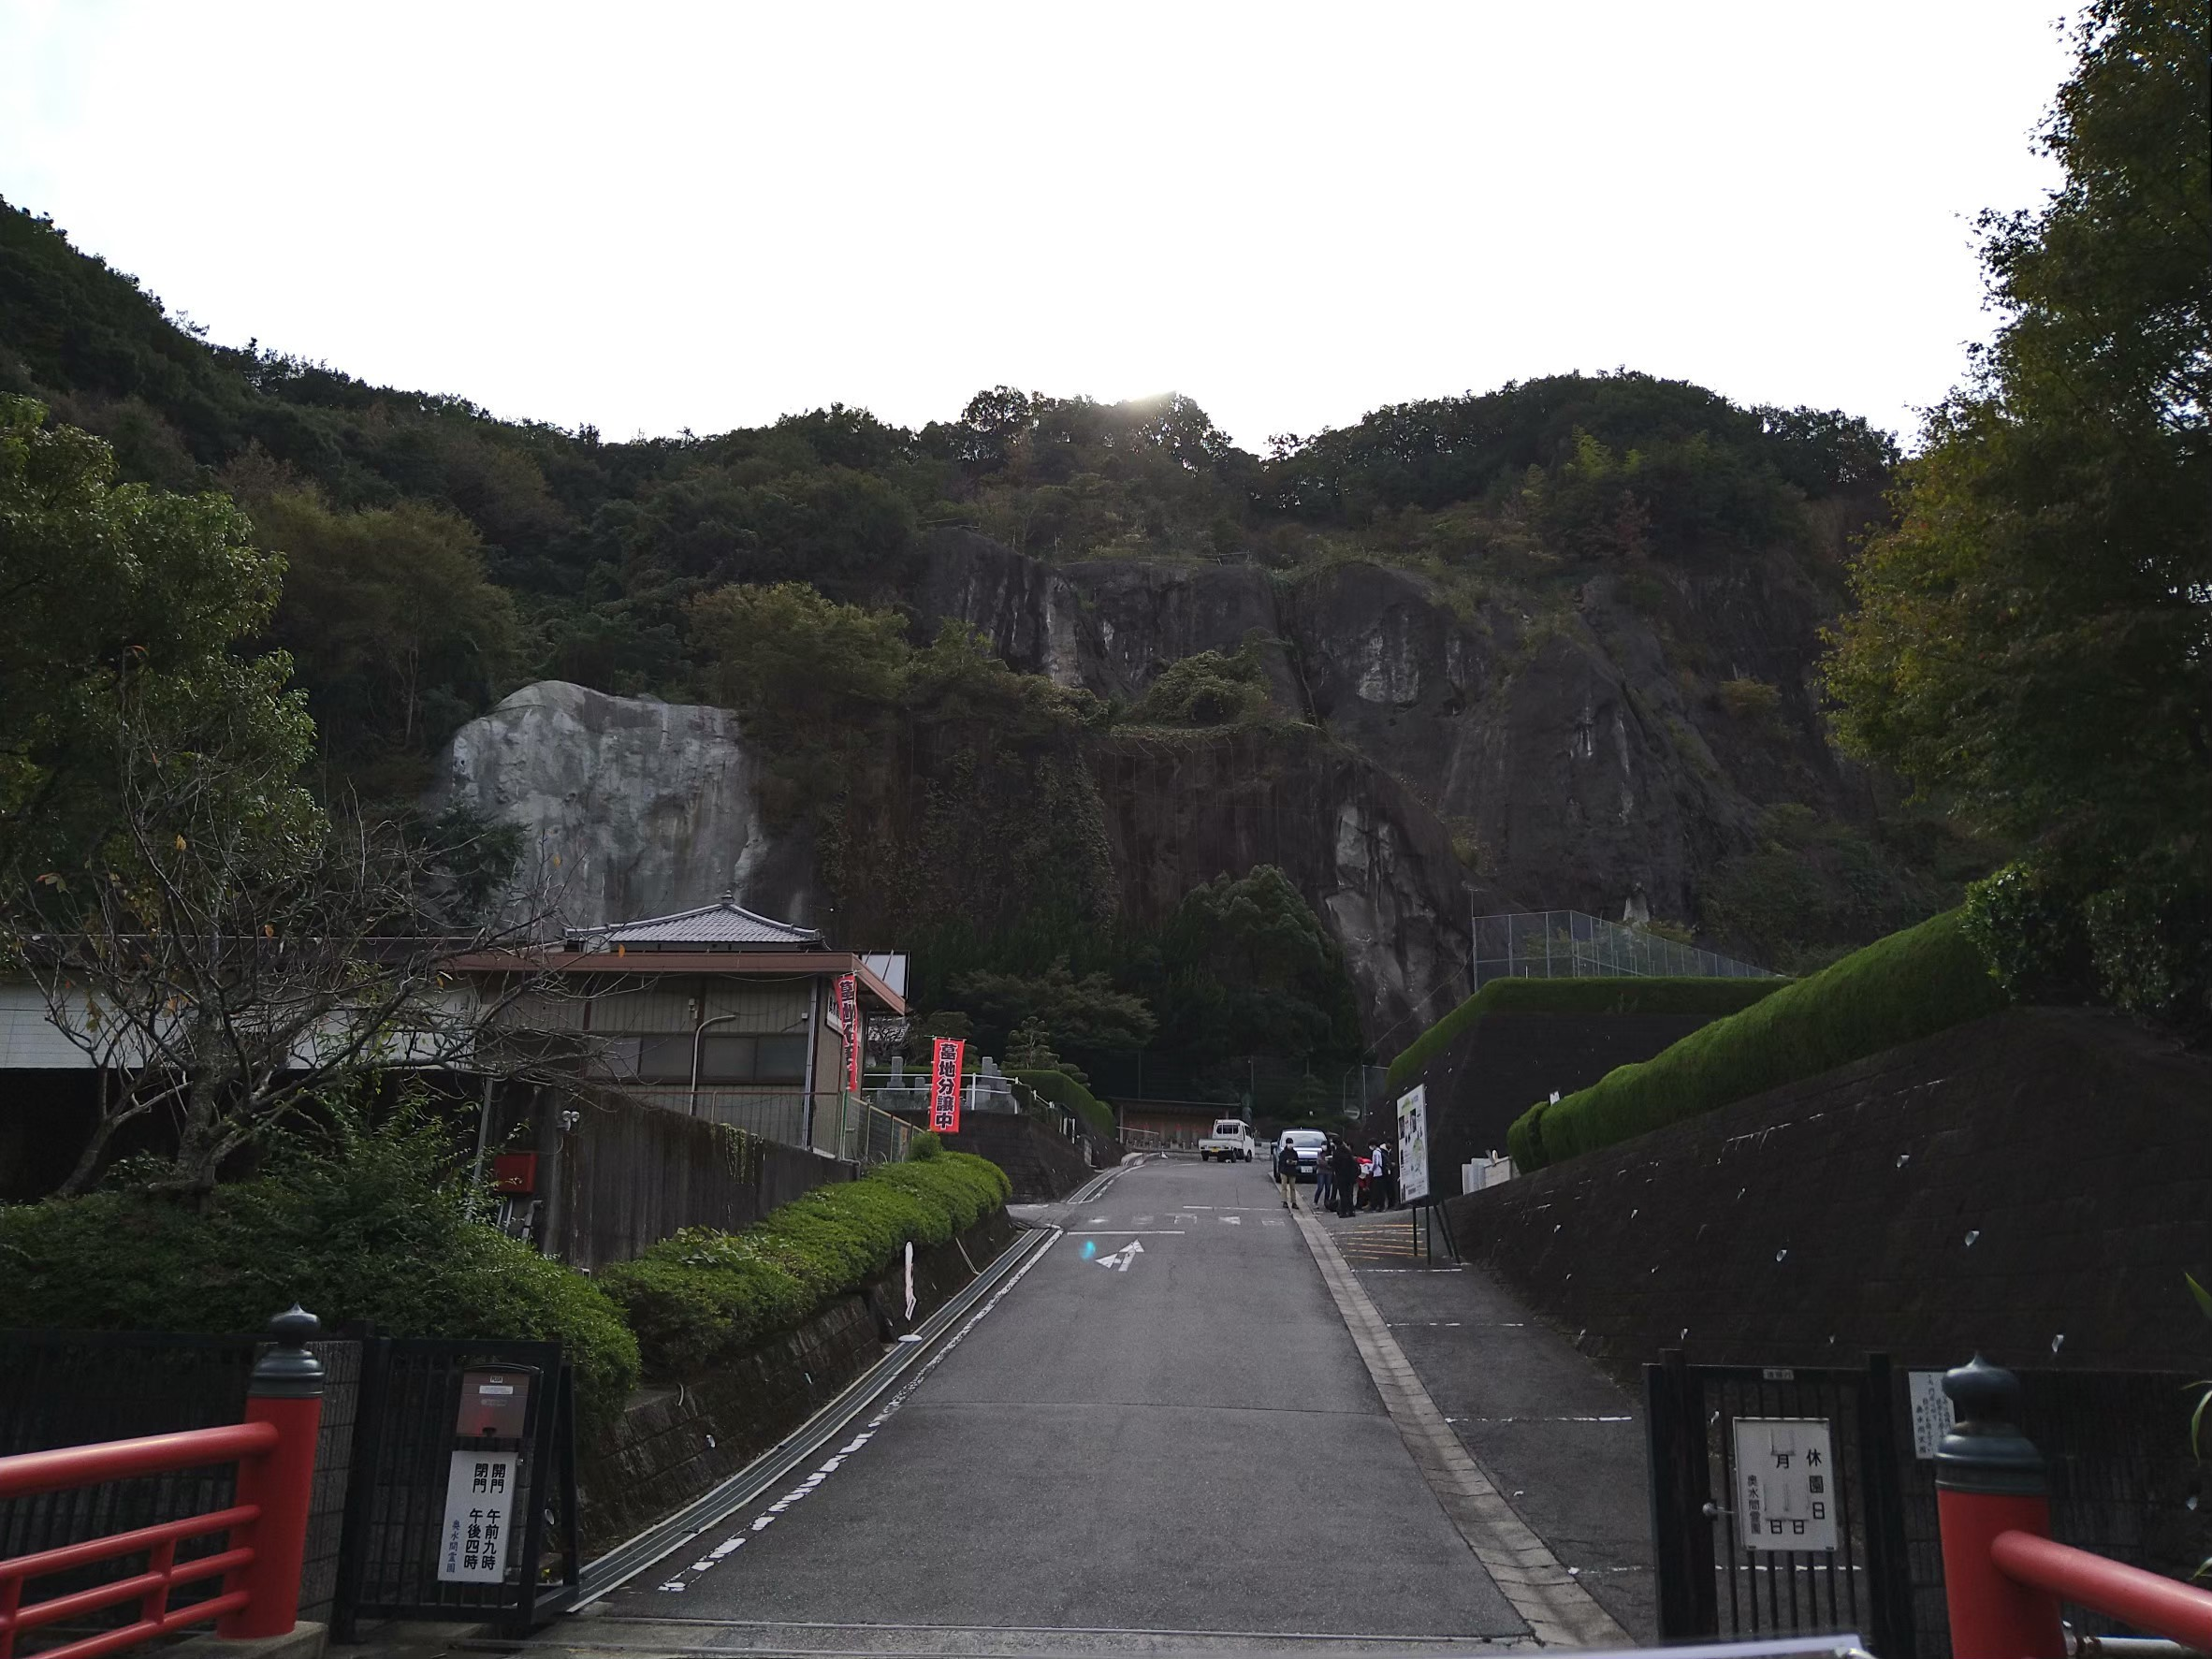
\includegraphics[scale=0.07]{files/地学実習/地点18.jpg}
      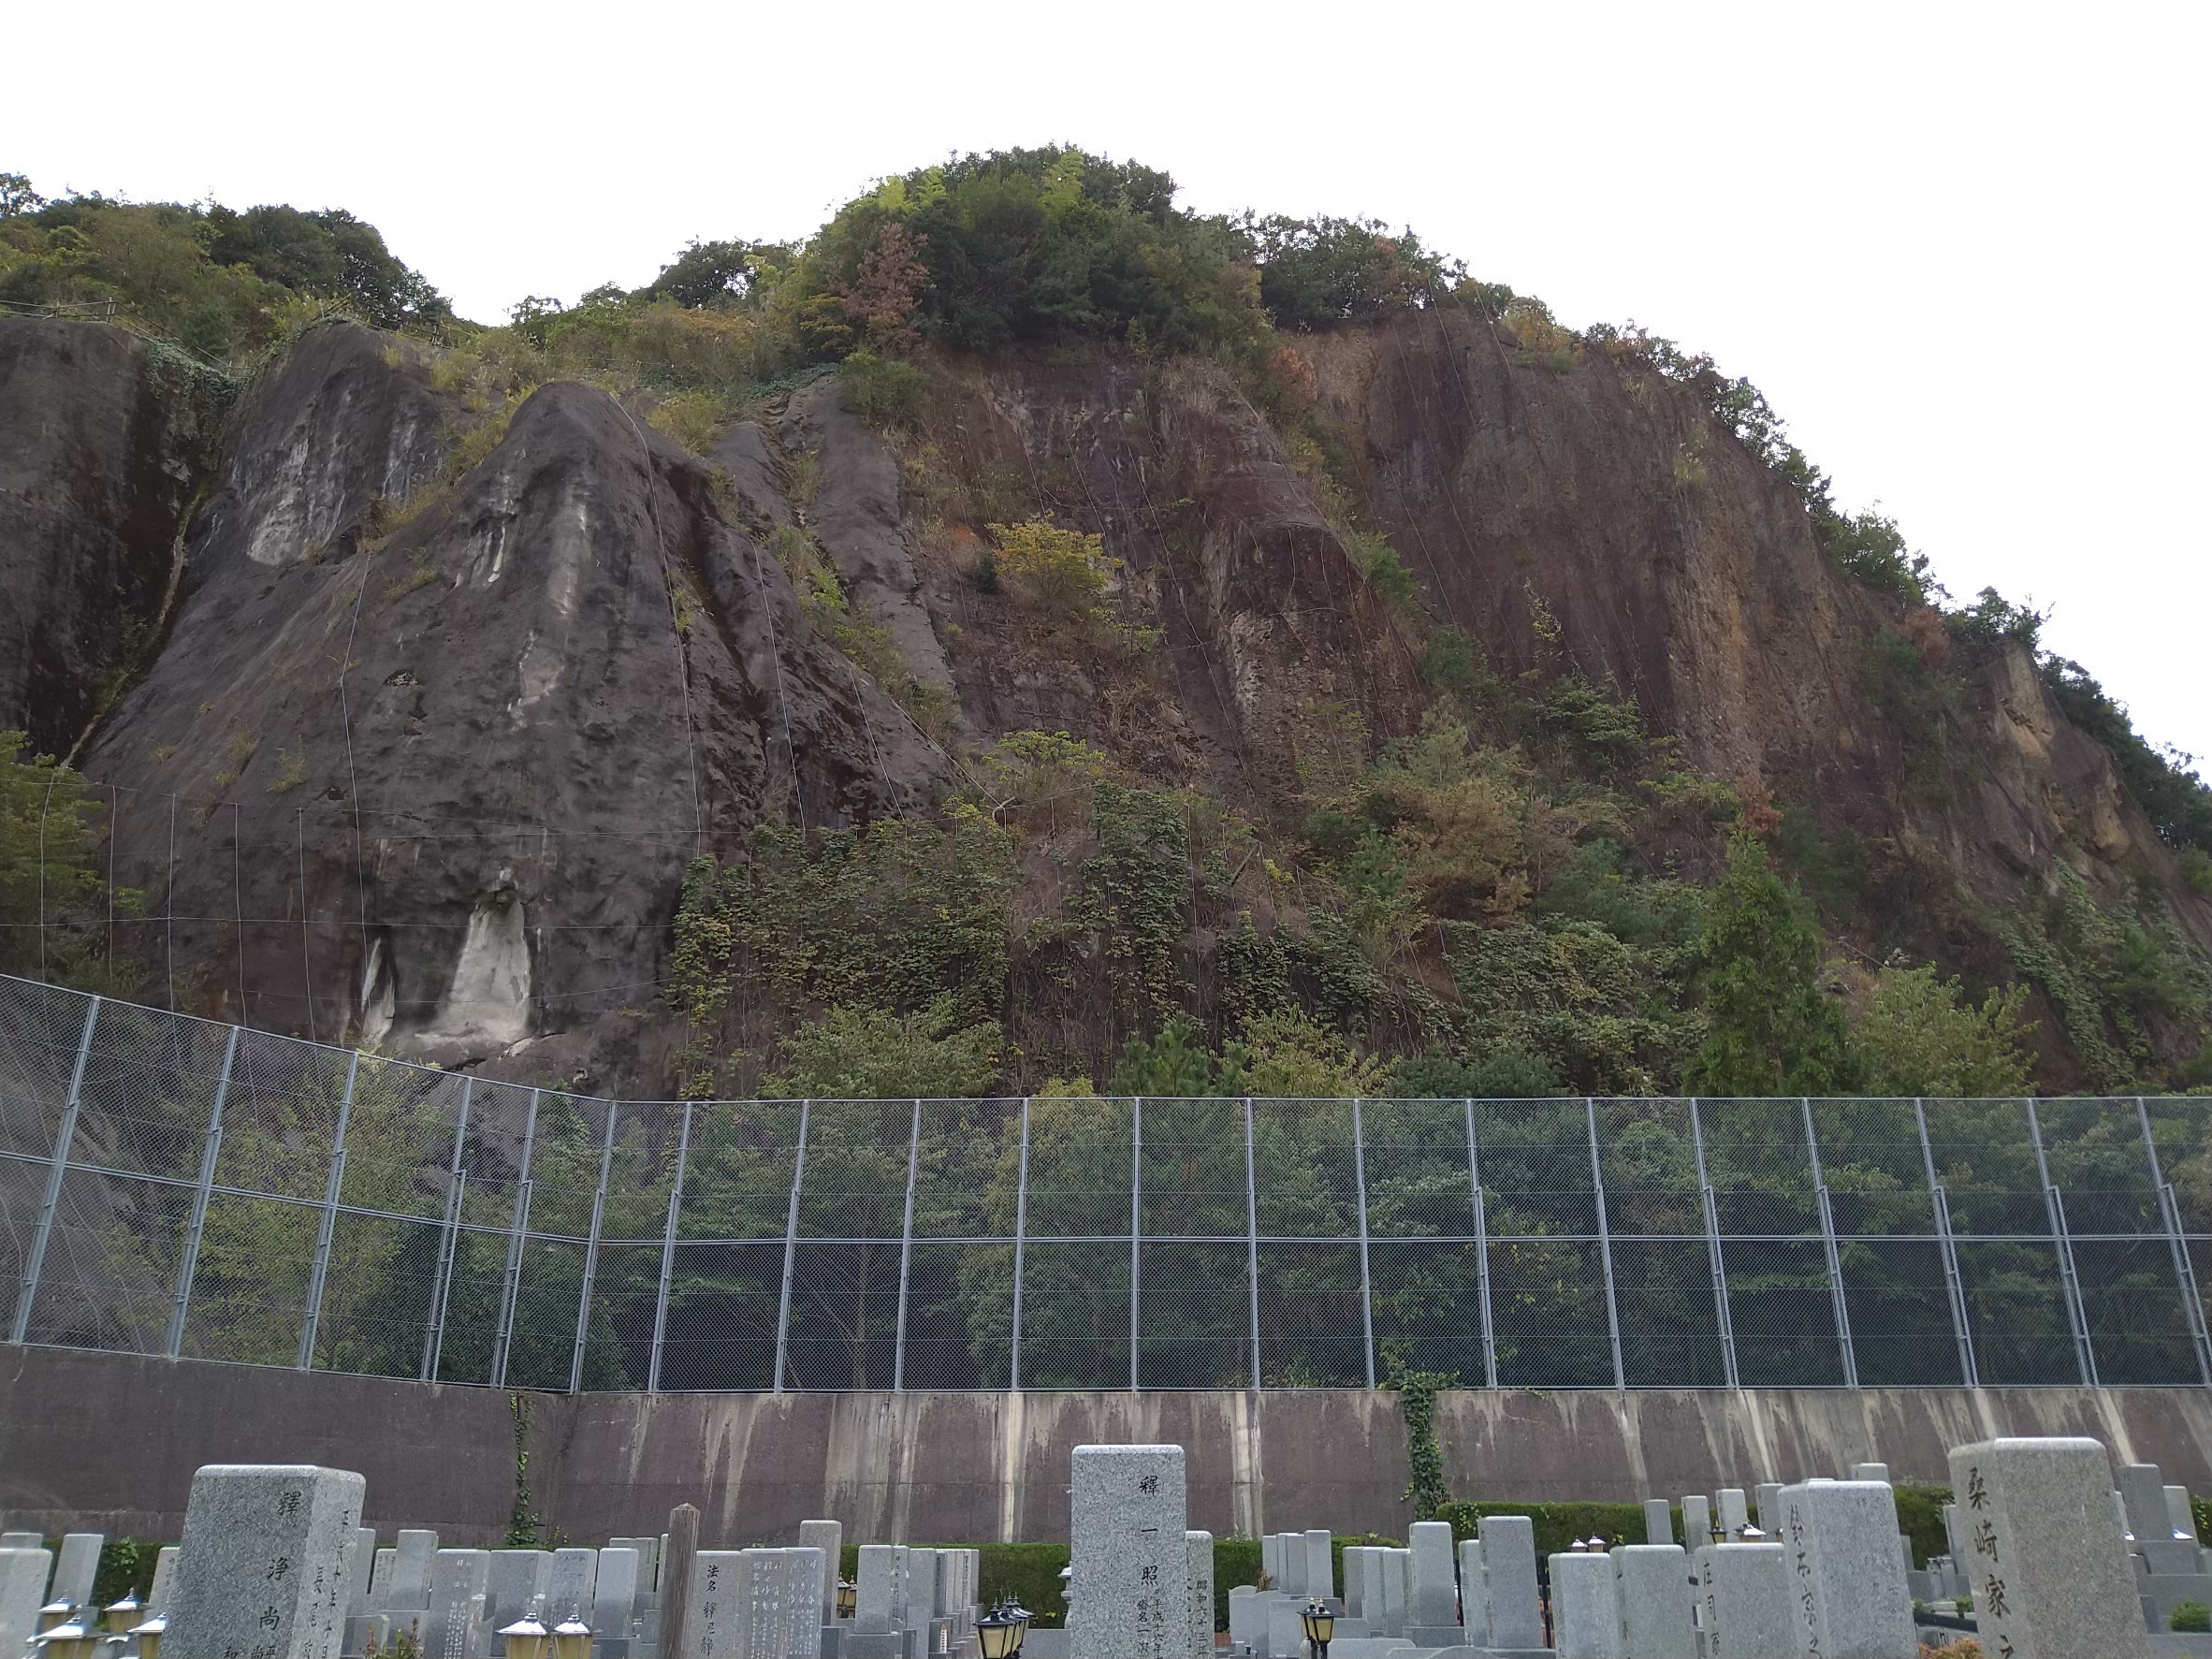
\includegraphics[scale=0.1]{files/地学実習/地点18_2.jpg}
      \caption{地点18(奥水間霊園)}
    \end{center}    
  \end{figure}
  \clearpage

  \section{地点19}
    \subsection{基本情報}
    岩石:泉南流紋岩
    \subsection{設問}
    \leftline{\large \textbf{◎露頭を構成する岩石を調べる。}}
    泉南流紋岩
%    \subsection{考察}
  \clearpage

  \chapter*{参考文献}
  \addcontentsline{toc}{chapter}{参考文献}
  \begin{flushleft}
    ・ニューステージ地学図表(浜島書店,2013)\par
    ・コトバンク『断層破砕帯』(\url{https://kotobank.jp/word/断層破砕帯-95225})\par
    ・コトバンク『扇状地』(\url{https://kotobank.jp/word/扇状地-88386})\par
    ・コトバンク『ケスタ』(\url{https://kotobank.jp/word/ケスタ-59426})\par
    ・大阪府 地形・地質(\url{https://www.pref.osaka.lg.jp/attach/21490/00148206/P41-42tikeitisitu.pdf})\par
    ・徳島の自然と歴史ガイドNo.3 和泉層群(\url{https://museum.bunmori.tokushima.jp/bb/chigaku/fossils/Izumi.html})\par
  \end{flushleft}

  
  \chapter*{謝辞と感想}
  \addcontentsline{toc}{chapter}{謝辞}
  このレポートは組版処理システムである\LaTeX で書いています。\LaTeX とその解説記事、ありがとう。\par
  タイトルはDeepLに訳してもらいました。ありがとう。\par

  このレポートは書くのがとてもしんどかったです。とはいえ地学野外実習はとても楽しかったし、レポートを書くのもなんやかんや楽しくはありました。ちなみに、後になるほど疲れでメモが減っていて書く内容もなくなっていったので、後半はとても困りました。あと、芸術点を狙って最初はドイツ語にでもしようかなと思っていたんですが、面白みがないのでやめました。

  特に書くことが無いので新世紀エヴァンゲリオンの名言を書いて〆たいと思います。\\

  \centerline{\textbf{父に、ありがとう。母に、さようなら。そして全ての子供達におめでとう。}}\par


\end{document}